% !TeX program = xelatex
\documentclass[11pt,a4paper]{article}
\usepackage[UTF8,fontset=fandol,scheme=plain]{ctex}
\usepackage[margin=25mm,top=24mm,bottom=25mm]{geometry}
\usepackage{amsmath,amssymb,amsthm,mathtools}
\usepackage{graphicx,booktabs,threeparttable,tabularx,array,longtable}
\usepackage{enumitem,algorithm,algpseudocode,microtype}
\usepackage[numbers,sort&compress]{natbib}
\usepackage{xcolor,xurl}
\usepackage[colorlinks=true,linkcolor=black,citecolor=black,urlcolor=blue!45!black,
  bookmarksnumbered=true,pdftitle={协议诱导的因果前沿：Release–Acquire 观测的精确支持编译}]{hyperref}
\usepackage{bookmark}
\usepackage{caption}
\captionsetup{font=small,labelfont=bf}
\renewcommand{\figurename}{图}
\renewcommand{\tablename}{表}
\renewcommand{\refname}{参考文献}
\renewcommand{\abstractname}{摘要}
\floatname{algorithm}{算法}
\algrenewcommand\algorithmicrequire{\textbf{输入：}}
\algrenewcommand\algorithmicensure{\textbf{输出：}}
\setlength{\parindent}{2em}
\setlength{\parskip}{.2em}
\linespread{1.12}
\setlength{\emergencystretch}{2em}
\setcounter{topnumber}{3}
\renewcommand{\topfraction}{.92}
\renewcommand{\textfraction}{.06}
\renewcommand{\floatpagefraction}{.8}
\newtheorem{theorem}{定理}[section]
\newtheorem{lemma}[theorem]{引理}
\newtheorem{corollary}[theorem]{推论}
\newtheorem{proposition}[theorem]{命题}
\theoremstyle{definition}
\newtheorem{definition}[theorem]{定义}
\renewcommand{\proofname}{证明}
\newcommand{\SB}{\mathsf{sb}}
\newcommand{\rf}{\mathsf{rf}}
\newcommand{\co}{\mathsf{co}}
\newcommand{\hb}{\mathsf{hb}}
\newcommand{\fr}{\mathsf{fr}}
\newcommand{\eco}{\mathsf{eco}}
\newcommand{\init}{\mathsf{init}}
\newcommand{\Cov}{\operatorname{Cov}}
\newcommand{\Supp}{\operatorname{Supp}}
\newcommand{\Lit}{\operatorname{Lit}}
\newcommand{\irr}{\operatorname{irr}}
\newcommand{\DAG}{\mathcal{D}}
\newcommand{\RF}[2]{\mathsf{RF}(#1,#2)}
\newcommand{\CO}[2]{\mathsf{CO}(#1,#2)}
\newcommand{\W}{\mathsf W}
\newcommand{\R}{\mathsf R}
\newcommand{\SAT}{\mathsf{SAT}}
\newcommand{\UNSAT}{\mathsf{UNSAT}}
% Generated from frozen JSON; do not edit.
\newcommand{\HistoryFour}{0.2223}
\newcommand{\HistoryThirtyTwo}{5.6706}
\newcommand{\BufferEightBTwo}{0.7028}
\newcommand{\BufferEightBD}{11.8927}
\newcommand{\BufferRatio}{16.9}
\newcommand{\BufferSparseBD}{0.1572}
\newcommand{\BufferSparseBTwo}{0.1741}
\newcommand{\BufferDenseBD}{0.2448}
\newcommand{\BufferDenseBTwo}{0.1882}

\title{\bfseries 协议诱导的因果前沿：\\[.3em]Release--Acquire 观测的精确支持编译}
\author{}
\date{}
\begin{document}
\maketitle
\vspace{-2.2em}
\begin{abstract}
不完整的来源观测会留下多个读自关系与修改序补全，分析任务因而需要回答条件下哪些来源和写序仍然可行，而不仅是寻找一个见证。困难在于：每个完成的执行图具有小接口，并不保证所有候选的共同表示也具有小接口。本文研究固定事件的 Release--Acquire 观测，提出由协议共同因果关系定义的未决前沿。对于前沿以外已经确定先于未来相关访问的历史，每个地址只需保留少量极大写；结合线程尾事件，可构造覆盖全部 RF／CO 候选的连续处理计划。我们从单生产者／单消费者缓冲的容量反馈及重置／唤醒屏障推导统一证书，并证明精确编译对全部原始赋值保持投影，使已退休事件的来源身份仍可用于条件支持与假设撤销。实验中，容量为三的分支缓冲从四轮增至三十二轮时，最大可达层状态保持为三十；容量增至六则触及当前状态预算。组件分解和日志快照频率又会改变编译与 SAT 的收益关系。这些结果说明，协议结构能够支持可复用的精确分析，同时给出其计算收益的具体适用条件。
\end{abstract}

\section{引言}
一条并发日志记录“读到了值 $1$”，通常没有记录它来自哪次写入。如果同一线程多次发布值 $1$，早、晚两次发布可能对应不同的同步知识：早发布发生在某次数据写之前，晚发布发生在它之后。加入“此次读来自晚发布”的假设，可能迫使另一个地址上的写序方向；撤销这条来源记录，先前排除的方向又应恢复。定位不一致日志、枚举一个字段的替代解释，以及比较候选来源，都需要反复回答这类条件问题。

一次可满足性求解提供一个完整见证，无法直接说明其余来源是否也可行。对每个新条件重新搜索全部支持虽然精确，却可能重复处理同一组同步约束。将固定观测的完成空间预编译为可复用表示，是一种自然选择。它的主要障碍不是如何在图上做一次可达性，而是如何在尚未选择读源和修改序时，控制要表示的整个候选空间。

这项困难具有明确的量词差异。为每个完成分别寻找一个小分解，允许布局依赖已选来源；查询表示却需要在未来假设未知时保留所有合法选择。同一批同值写和读可以使每个完成的 RF 图很窄，而所有候选取并后形成完全二部图。已有基于完成图的结构保证因而不能直接作为统一编译接口的保证。

本文利用同步协议所建立的\emph{共同因果关系}。即使一个读的具体来源未定，所有候选来源仍可能具有同一个前序。随着编译推进，某些历史事件已确定先于未来每个相关访问。对于这部分稳定历史，一个旧写若被同地址的更晚稳定写覆盖，就不可能再作为未来读的来源，也不可能是未来写的固定修改序覆盖前驱。剩下的稳定极大写，每个地址至多有线程数那么多个。必须继续显式保留的其他事件集中在未决因果前沿中。

由此得到本文的结构定理：若未决前沿至多有 $c$ 个事件，线程数为 $p$，地址数为 $a$，则整个 RF／CO 候选图有可直接构造的处理计划，最大事件袋大小至多 $c+ap+p+a+1$。这里界定的是所有候选共同使用的接口，允许一条 RF 或 CO 覆盖边跨过任意长历史。事件退出接口后，其关系作用由联合摘要保存；它曾选择的原始文字仍保留在编译路径上。安全遗忘关系状态与保留历史查询身份因而可以同时实现。

结构参数还必须能从程序纪律推出。我们给出两种具体来源。双模索引缓冲的容量反馈限制所有尝试的来源窗口，上界通过真实前缀中的因果环反证得到，无需等待完整日志的末端。星形汇聚／唤醒屏障则利用重置写推动到达来源前进，再经反馈锁定当前调用；适当布局使任意多失败轮询不增加未决前沿。两个协议构造保留完整有限前缀，并为尚未选定的 RF／CO 提供同一证书和计划。

本文的贡献集中于三个联系。第一，证明共同因果前沿与稳定极大写如何约束整个候选图，并明确二元选择及连续生存期所需条件。第二，给出反馈缓冲和屏障的可检查协议推导，以及失败读链和地址封闭组合的构造，从程序参数获得接口界。第三，将这一结构接到精确原始投影和完整支持查询上，以实现及冻结实验说明反复查询的收益何时出现、何时被组件缓存或构造成本抵消。通用关系分析、自动机检查、知识编译及单字段修复分别作为这些联系的基础和使用方式。

实验中的正面结果与边界同样影响结论。固定容量的缓冲在所测历史增长下保持小的可达层状态，并保留跨阶段来源关联；更大容量会使联合状态迅速增加。屏障中的可提取组件让局部缓存有效应对大量新全局条件，而实际日志诊断中，快照频率足以改变编译与 SAT 的端到端排名。本文据此研究一种结构可解释的支持编译方法，而不以普遍性能领先作为理论前提。

\section{背景与预备知识}\label{sec:background}
\subsection{Release--Acquire 执行关系}
一次共享内存访问表示为一个带身份的事件，记录所属线程、地址及读写类型。写 $\W(x,v)$ 向地址 $x$ 写值 $v$，读 $\R(x,v)$ 观测值 $v$。本文采用固定事件的 RA 片段：全部非初始化写为 release 写，全部读为 acquire 读；地址和写值已经确定。片段不含 RMW、fence、非原子访问或动态事件激活。每个地址有一个初始化写，所有非初始化事件组成若干线程序列。$\SB$（sequenced-before）表示各线程的严格程序顺序；实现可存其邻接边。

读自关系 $\rf$（reads-from）为每个读指定唯一的同地址写来源，并要求返回值满足该读的观测。两个写即使写入相同值，也具有不同身份，可以成为不同来源。修改序 $\co$（coherence order）在每个地址的所有写上给出严格全序，初始化写最小；它不比较不同地址的写。给定这些关系，就得到一个候选完成的执行图。

在所选片段中，读自边建立 release/acquire 同步，因果关系为
\begin{equation}\label{eq:hb}
 \hb=(\SB\cup\rf\cup\init)^+.
\end{equation}
$\init$ 将每个初始化写连到全部非初始化事件。上标 $+$ 表示非空传递闭包，因此 $\hb(e,f)$ 表示存在一条由程序顺序、同步和初始化边组成的非空路径。稀疏实现只需把初始化连到各线程首事件，再沿线程边传播。

读源和修改序还确定读取相对于更晚写的顺序。若 $r$ 读取 $w$，且 $w<_{\co}v$，则 $r$ 位于 $v$ 之前的 from-read 关系中。用关系复合 $;$ 表示先沿左关系再沿右关系，有
\begin{equation}\label{eq:eco}
 \fr=\rf^{-1};\co,\qquad
 \eco=(\rf\cup\co\cup\fr)^+.
\end{equation}
$\eco$ 汇合了同地址的读源、写序和读后写关系。本文的 RA 合法性条件为
\begin{equation}\label{eq:ra}
 \irr(\hb;\eco^?).
\end{equation}
上标 $?$ 表示加上恒等关系，$\irr$ 要求不存在从某个事件回到自身的关系对。因此式~\eqref{eq:ra} 同时排除 $\hb$ 自环，以及一条因果路径接上一条同地址一致性路径所形成的闭环。这是本文随后证明和实现共同使用的语义；RA 一致性检验中相应的读／写一致性条件可见~\cite{tunc2023}。

一个具体冲突说明这条公理如何过滤来源。若 $w\mathrel\rf r$、$w<_{\co}v$ 且 $v\mathrel\hb r$，则 $r\mathrel\fr v$，与 $v\mathrel\hb r$ 构成闭环。也就是说，读不能从一个已经被其因果前序写覆盖的旧写取值。同线程有序读取的来源也不能沿修改序倒退。这样的 coherence 约束让共同因果关系限制来源选择，具体推导在协议证明中展开。

\subsection{图分解与活跃接口}
处理候选图时，我们用一列事件集合 $B_0,B_1,\ldots$，称为\emph{袋}。它们覆盖所有事件，每条需要处理的边的两个端点至少在一个袋中共存，并且一个事件出现的袋下标形成连续区间。这是图分解的覆盖与连通性要求在线性袋序列上的形式~\cite[§3.1]{conrado2026}，称为路径分解。我们用 $K=\max_i|B_i|$ 表示最大事件袋大小；传统路径宽度为 $K-1$。编译器在处理边时保留袋中的事件关系，事件最后一次离开袋后，通过摘要保留其对未来的影响。

接口大小取决于同时活跃的端点数。一个旧写即使与很远以后的读相连，也只需要持续保留这一个端点；许多彼此不同的旧端点同时连接未来才会增大袋。对严格偏序 $L$，其覆盖关系定义为
\[
 \Cov(L)=\{(u,v)\in L:\nexists z.\ L(u,z)\land L(z,v)\}.
\]
有限偏序满足 $\Cov(L)^+=L$。这允许后文用稀疏边生成已经确定的修改序，而不把传递闭包的每一对都变成必须共存的端点。

\subsection{条件查询与知识编译}
设布尔函数 $F(X)$ 表示一组可行选择。对部分赋值 $\alpha$ 条件化，就是研究 $F\land\alpha$ 的模型；撤销一项假设则恢复相应选择。一个满足赋值可以回答“一种可行选择是什么”，却不能直接回答哪些变量取值在\emph{某个}模型中可行、哪些在\emph{所有}模型中必然成立。知识编译把构造费用前置，将 $F$ 转为支持所需查询的显式表示~\cite{darwiche2002}。

若表示引入辅助变量 $Y$，所需的精确性是 $F(X)\equiv\exists Y\,A(X,Y)$：辅助状态可以隐藏，原始选择不能丢失。这个等式同时保证每个原始模型都能扩展到表示中，以及表示不会引入新的原始模型。第~\ref{sec:compilation}节将对具体编译表示证明这种双向保证。

\section{问题定义与方法概览}\label{sec:problem}
\subsection{同值发布为什么需要保留身份}\label{sec:example}
考虑一个双线程、两轮的重复发布实例。线程 A 每轮先写 $x$，发布一次标志 $fa$，再写 $y$，随后再次发布同一标志值；线程 B 对称地先写 $y$，发布 $fb$，再写 $x$，再次发布 $fb$。两者接着读对方的标志并读取本线程先写的数据地址。数据写值均为 $1$，第一、二轮标志分别写 $1,0$；对应等待读分别观测 $0,1$。附录~\ref{app:witness} 列出所有事件和合法完成。与当前查询相关的事件是
\[
\begin{aligned}
 A\text{ 第1轮}:&\quad \cdots\ a_0=\W(fa,1)\ ;\ u=\W(y,1)\ ;\ a_1=\W(fa,1)\ \cdots,\\
 B\text{ 第2轮}:&\quad v=\W(y,1)\ ;\ \cdots\ ;\ r=\R(fa,1)\ ;\ s=\R(y,1).
\end{aligned}
\]
这是一段发布内核的有限观测，用来展示查询语义。第~\ref{sec:protocols}节的循环缓冲与屏障另有可追溯的协议来源。

令 $d=\RF vs$，$e=\RF{a_0}r$，$l=\RF{a_1}r$，$q=\CO uv$。在假设 $d\land l$ 下，有
\[
 u\mathrel{\SB}a_1\mathrel\rf r\mathrel{\SB}s,
\]
所以 $u\mathrel\hb s$；由 WR 一致性和 $s$ 的来源 $v$ 得到 $q$。于是 $d\land l\land\neg q$ 不可满足。若将来源换为早发布 $a_0$，这一因果路径消失，而且 $d\land e\land\neg q$ 确有合法完成；$d\land e\land q$ 也有合法完成。两种标志来源写入相同值，却对另一个地址的 CO 支持产生不同影响。撤销 $l$ 后，$d$ 下两个 CO 方向恢复支持。这里“恢复”有完整见证，而不只是一个静态近似没有删掉某个方向。

这个交互同时要求两种信息。$a_0$ 位于 $a_0$ 和 $a_1$ 的共同因果前缀，无论 $r$ 选择哪一个，$a_0$ 都先于 $r$；这种共同事实可以永久使用。但 $u$ 只先于晚发布，分析不能把两个来源身份合成一个事件，也不能把当前查询推得的 $u\mathrel\hb r$ 永久写入基础表示。

\subsection{固定观测与完整支持}
输入 $I$ 包含事件集合 $E$、线程顺序、事件类型与固定地址、写值、初始化、观测 $O$，以及可检查的程序位置和协议元数据 $\Lambda$。令 $n=|E|$，线程数为 $p$，地址数为 $a$。每条线程记录是所声明程序的无缺口有限前缀，允许在调用内部或等待中停止，全部失败尝试保留。$\Lambda$ 指明线程角色、协议地址所有权、调用位置、容量或参与者数及必要的布局约定；它在选择 RF／CO 前给出。本文不从任意无注释日志自动发现协议。

我们区分两类输入精度。完整值观测记录每次读值及已发生分支。分支观测允许某些返回值只由允许集合或已发生守卫约束。例如缓冲成功消费只说明两个索引不同，不能把未记录的对端返回值补成某个版本。写的具体地址与写值在两种模式中均已由固定事件前缀确定。

在任何协议过滤之前建立原始变量集合 $X$。每个读与所有满足其原始值观测的同地址写之间注册一个 RF 位；未记录值的读包含所有同地址写。对每个同地址无序写对注册一个 CO 方向位，反方向用该位的否定表达。初始化相关位也在内。后续证明某个位恒真或恒假时，只记录其常量，不删除或重编号。令 $\Phi_I(X)$ 为“恰一来源、逐地址初始化最小的全修改序、全部值／分支观测及式~\eqref{eq:ra}”的布尔函数。

\begin{definition}[条件完整支持]\label{def:support}
对原始文字合取 $\alpha\subseteq\Lit(X)$，若 $\Phi_I\land\alpha$ 可满足，则
\[
 \Supp_I(\alpha)=\{\lambda\in\Lit(X):\exists x.\ \Phi_I(x)\land\alpha(x)\land\lambda(x)\}.
\]
若不可满足，接口单独返回 $\UNSAT$。在可满足时，$\lambda$ 必然成立等价于其反文字不在支持集合中。
\end{definition}

返回集合涵盖全部原始 RF 和 CO 位，含已退休事件及永久常量。目标是对同一个固定 $I$ 反复增加和撤销 $\alpha$，不因条件变化而丢失原来可能的完成。

\subsection{先固定结构，再接受查询}
构造分两部分进行。协议分析从输入中推出可靠来源域 $D$、共同因果下界 $H$ 和共同写序下界 $L$，生成证书 $\Gamma_I$；在这些候选上建立 $G_I$ 及处理计划 $\pi_I$。随后精确编译得到 DAG $\DAG_I$，由它回答任意 $\alpha$。顺序可概括为
\begin{equation}\label{eq:quantifier}
 \exists(\Gamma_I,G_I,\pi_I)\quad
 \forall J\text{ 合法完成}\quad
 \exists\gamma_J:\ J\text{ 可由同一计划表示}.
\end{equation}
证明注释 $\gamma_J$ 可以记录该完成选了哪次发布及未记录的实际读值；调用编号、失败串位置和计划不能随 $J$ 改变。后续投影定理还会排除表示中的非法完成，因而比式~\eqref{eq:quantifier} 的覆盖条件更强。

共同前序是这一步的关键。例如 $a\mathrel\SB b$，且一个读可选同值来源 $a$ 或 $b$，虽然没有必选 RF，两个完成中都有 $a\mathrel\hb r$。只把必选 RF 加入 $\SB$ 再闭包会漏掉它。第~\ref{sec:frontier}节从这样的可靠关系定义未决因果前沿，并证明其余仍需连接未来的稳定写每地址至多保留 $p$ 个。第~\ref{sec:protocols}节解释如何由协议获得足够强的关系与连续计划；第~\ref{sec:compilation}节则证明关系状态的压缩不影响原始条件支持。

\section{因果前沿与整个候选图的接口}\label{sec:frontier}
一个已处理事件可能仍与许多未来事件相连。若这些连接都指向同一个旧写，保留这个写就足够；若许多旧事件分别有未处理连接，接口才会增长。本节用已经认证的共同因果关系区分这两种情况，并同时处理尚未选择的来源和写序。

\subsection{可靠关系与可检查的来源过滤}
证书 $\Gamma_I$ 包含每个读的候选域 $D(r)$、共同因果关系 $H$、逐地址写序下界 $L$、推导记录，以及原始变量的归属信息。对每个合法完成 $J$，它满足
\begin{equation}\label{eq:reliable}
 \rf_J^{-1}(r)\in D(r),\qquad H\subseteq\hb_J,\qquad L\subseteq\co_J.
\end{equation}
这里 $H$ 和 $L$ 都是严格传递关系，$H$ 包含 $\SB$ 和初始化先行关系，$L$ 只含同地址写对，并包含 $H$ 的同地址写限制及初始化最小关系。$D$ 是所有合法来源的上近似；其中每个元素未必最终有支持。

我们要求证书对下列必要条件达到饱和。若 $H(r,w)$，从 $D(r)$ 删除 $w$；否则选择该来源会形成 $\hb$ 环。若存在同地址写 $z$，使 $L(w,z)$ 且 $H(z,r)$，也删除 $w$；否则 $r\mathrel{\fr}z\mathrel{\hb}r$ 违反一致性。下文分别称这两条为 R1 和 R2。若 $D(r)=\{w\}$，则把 $(w,r)$ 加入 $H$，称为 R3。共同前序规则为
\begin{equation}\label{eq:rall}
 \frac{D(r)\ne\varnothing\quad
       \forall w\in D(r).\ (u=w\ \lor\ H(u,w))}{H(u,r)}\quad(R_{\forall}).
\end{equation}
该规则只引用此前得到的事实。任取合法完成，它为 $r$ 选择的来源 $w$ 仍在 $D(r)$；于是 $u$ 先于该写或等于该写，再经实际 $\rf(w,r)$ 到达 $r$。这证明结论对所有完成成立，且没有把任何候选选成必选来源。

R1--R3 和式~\eqref{eq:rall} 的可靠性属于关系分析的基本推理~\cite{haas2023}。这里需要它们提供的是下一定理的具体前提：稳定写若已被更晚的稳定写覆盖，其所有未来来源候选必须已经删除。只保存来源域而不实施 R2，不能得到这个结构结论。

\subsection{前沿、稳定写与真实候选边界}
令 $\theta$ 为所有非初始化事件的一个线性排列，保持每个线程的 $\SB$。它决定编译时引入事件的次序。令 $P_t$ 为前 $t$ 个事件，$Q_t$ 为其余事件。两个事件称为\emph{相关}，当且仅当它们访问同一地址且至少一个是写。定义
\begin{equation}\label{eq:frontier}
 U_t=\{e\in P_t:\exists f\in Q_t,\ e,f\text{ 相关且 }\neg H(e,f)\},
 \qquad c=\max_t |U_t|.
\end{equation}
$U_t$ 是未决因果前沿。事件 $e\notin U_t$ 表示其与每个未来相关访问的先后已经确定；即使 $e$ 很早出现，也可能仍是未来读取唯一需要的旧写。

对地址 $x$，令 $S_x(t)$ 为 $P_t\setminus U_t$ 中访问 $x$ 的写，令 $M_x(t)$ 为其中关于 $H$ 的极大元素。记 $M_t=\bigcup_x M_x(t)$，并以 $T_t$ 表示每个线程在 $P_t$ 中的最后一个事件。一个线程内的同地址写按 $H$ 全序排列，因此
\begin{equation}\label{eq:maxwrites}
 |M_x(t)|\le p,\qquad |M_t|\le ap,\qquad |T_t|\le p.
\end{equation}
极大性在这里相对于\emph{稳定写}，不是相对于所有已引入写。一个仍在前沿中的新写不能用来代替更老的稳定写。

构造无向候选事件图 $G_I$。它含全部 $w\in D(r)$ 对应的 RF 边、$L$ 中不可比较的每个同地址写对、$\Cov(L)$ 的边、真实线程邻接边，以及每个初始化写到各非空线程首事件的边。不可比较写对以后选择两个 CO 方向之一；$\Cov(L)$ 为固定 CO 提供稀疏生成边。$H$ 和 $L$ 的稠密闭包用于推理，但不作为候选图的全部边加入。令
\[
 F_t=\{e\in P_t:\exists f\in Q_t,\ \{e,f\}\in E(G_I)\}
\]
为非初始化事件的真实候选边界。它直接决定哪些旧事件还有未处理关联。

\begin{theorem}[因果前沿控制统一候选图]\label{thm:frontier}
设 $I$ 含 $n$ 个事件、$p$ 个线程和 $a$ 个地址。设可靠证书 $\Gamma_I$ 满足上述传递性、包含关系及 R1/R2 饱和条件，$\theta$ 为预先固定的 $\SB$ 相容排列，$c$ 由式~\eqref{eq:frontier} 定义。则每个切口都有
\begin{equation}\label{eq:containment}
 F_t\subseteq U_t\cup M_t\cup T_t.
\end{equation}
从 $G_I$ 可直接构造一个覆盖全部候选二元选择的连续袋计划 $\pi_I$，其最大事件袋大小满足
\begin{equation}\label{eq:mainK}
 K\le c+ap+p+a+1.
\end{equation}
这个图和计划同时适用于 $I$ 的所有合法完成及所有后续原始变量查询。
\end{theorem}
\begin{proof}
固定切口，考虑 $e\in F_t\setminus U_t$ 的一条跨切口边 $\{e,f\}$。对于 RF 边有两种端点角色。若 $e$ 为过去的读而 $f$ 为未来的写，稳定性给出 $H(e,f)$，R1 已排除这个来源，所以该边不可能存在。若 $e=w$ 为过去的写、$f=r$ 为未来的读，并且 $w\notin M_t$，有限严格偏序中存在同地址稳定写 $z$，满足 $H(w,z)$。由证书包含关系有 $L(w,z)$；由 $z$ 的稳定性有 $H(z,r)$。R2 已删除 $w\to r$，同样矛盾。因此任何仍与未来读相连的稳定写都在 $M_t$ 中。

再考虑两个写端点 $w=e$、$v=f$。稳定性给出 $H(w,v)$，从而 $L(w,v)$；它们不可能是未决 CO 对。如果 $w\notin M_t$，仍取稳定写 $z$ 使 $H(w,z)$。因为 $v$ 在未来，有 $H(z,v)$，所以 $L(w,z)$ 和 $L(z,v)$ 同时成立。$z$ 严格位于二者之间，排除了 $(w,v)\in\Cov(L)$。故固定覆盖边的旧稳定端点也必须属于 $M_t$。这一步使理论允许跨很长历史的覆盖边：它保留少量极大写，而不要求每条边都短。

真实 $\SB$ 邻接边跨切口时，过去端点必为该线程在 $P_t$ 中的尾事件。因为 $\theta$ 保持线程顺序，不能已有另一个同线程事件越过这个未引入的直接后继。故该端点在 $T_t$ 中。初始化端点单独计入 $a$，不属于 $F_t$ 的计数。所有候选边类型已经覆盖，式~\eqref{eq:containment} 成立。

构造时先引入初始化写并连续保留。在引入 $\theta(t+1)$ 前保留真实边界 $F_t$；引入新事件后，处理以它为较晚端点的所有二元组，随后退休已经没有未来候选关联的事件。当前袋包含在
\[
 \{\text{初始化写}\}\cup F_t\cup\{\theta(t+1)\}
\]
中。结合式~\eqref{eq:maxwrites} 即得式~\eqref{eq:mainK}。每条边在其较晚端点引入时得到处理；每个事件从首次引入至最后关联连续存在。即使某个事件在不同切口的 $U_t$、$M_t$ 分类改变，也不会退休后重新引入，因为实际退休依据是 $F_t$。读的来源计数在其所有 RF 组处理完后检查。全部选择组、最后关联位置和计数检查位置只依赖证书与 $\theta$，不依赖选择了哪个完成或查询。\qedhere
\end{proof}

定理区分了两种压缩。关系推理删去永远不可能的候选；稳定写论证进一步说明，即便某些旧候选一直存在，整个过去仍只需少量代表与未来相连。变量身份随后保留在编译路径中，而事件关系可在接口外被摘要化。第~\ref{sec:compilation}节证明两者兼容。

\subsection{二元选择、阶段分隔与量词边界}
二元 RF 组只处理一个候选 $w\to r$ 的取舍，并在 $r$ 活跃期间累计已选来源数。若把一个读及其全部候选作为一次原子选择，它们必须同时出现在袋中，这超出了定理的二元边覆盖前提。例如一线程依次写 $w_1,\ldots,w_h$，另一线程只有读 $r$，所有写值都等于读值。在先引入 $r$ 的布局上，$c=1,p=2,a=1$；全部来源仍可行，一个原子 RF 组却有 $h+1$ 个非初始化端点。若另给来源域上界 $d=\max_r|D(r)|$，通过延长候选写生存期可得保守原子组界
\[
 K_{\rm atomic}\le c(d+1)+ap+p+a+1.
\]
附录~\ref{app:atomic} 给出相应调度证明。本文的主构造始终采用二元组。

许多协议更容易先证明按阶段的共同因果分隔。若阶段布局保持 $\SB$，每阶段最多 $b$ 个事件，且相隔至少 $h$ 个阶段的事件均有 $H(e,f)$，则切口的 $U_t$ 只可能来自最近 $h$ 个阶段，故 $c\le hb$。定理立即给出 $K\le hb+ap+p+a+1$。已有完整交替发布网络的来源块锁定证明可以产生 $h=2d+1$，其中 $d$ 为通信网络直径。由此，其接口界不再需要“每隔 $G$ 阶段必有一次写”的写覆盖假设：一个地址只在开始和很晚以后写入，中间反复读取，也只需保留稳定的极大写。该推论保留了原网络的完整交替观测前提；第~\ref{sec:protocols}节通过真实反馈给出适用于有限前缀的另一种分隔来源。

不能用“每个完成都存在小分解”替代定理中的同一候选结构。考虑一线程对同一地址写 $h$ 次相同值，另一线程连续读 $h$ 次该值。任何合法完成的来源编号按 RR 一致性非降。按写编号依次引入该写及从它读取的读，可用至多三个非初始化端点覆盖该完成的线程邻接与已选 RF 图。可是每对写、读都在某个 SC 完成中相连：把全部读放在指定写之后、下一写之前即可。因此全候选 RF 图包含 $K_{h,h}$，其任意路径分解的袋至少为 $h+1$。这展示的是量词顺序差异：逐完成选择布局不能控制候选并图。本文的协议论证必须在选择来源之前构造 $\Gamma_I,G_I,\pi_I$。

\section{从同步协议构造证书与处理计划}\label{sec:protocols}
定理~\ref{thm:frontier} 把问题转化为寻找可靠且较强的 $H$。本节研究两种已用于共享内存程序的同步机制：容量限制下的生产／消费反馈，以及所有参与者到达后的重置／唤醒。证明使用线程前缀和真实读写关系，不依赖有限日志最后一次读恰好锁定某个来源。阶段编号由程序位置确定，只用于推理和布局。

\subsection{双索引循环缓冲的反馈窗口}\label{sec:buffer}
GPS 的循环缓冲例子使用两个模索引控制单生产者和单消费者之间的槽复用~\cite{gps2014}。我们取其 Fig.~6 的控制结构，设有效容量为 $C\ge1$，数组长度及模数为 $m=C+1$，索引 $wp,rp$ 初始均为 $0$。生产者唯一写 $wp$，消费者唯一写 $rp$。一次生产尝试先读自身索引 $u\gets wp$，再读对端索引 $v\gets rp$；若 $(u+1)\bmod m=v$ 则返回满，否则执行槽写等至多 $B$ 个工作事件，再写 $wp\gets(u+1)\bmod m$。消费尝试先读 $u\gets wp$，再读自身索引 $v\gets rp$；若 $u=v$ 则返回空，否则执行槽读等工作事件，再写 $rp\gets(v+1)\bmod m$。工作代码不能访问两个控制索引。

下面伪代码中，所有共享读写分别使用 acquire 和 release；\texttt{payload} 只访问载荷地址。
\begin{center}
\begin{minipage}[t]{.48\linewidth}\small
\begin{verbatim}
try_put(value):
  u := load(wp)
  v := load(rp)
  if (u + 1) mod m = v:
    return FULL
  payload_put(u, value)
  store(wp, (u + 1) mod m)
  return OK
\end{verbatim}
\end{minipage}\hfill
\begin{minipage}[t]{.48\linewidth}\small
\begin{verbatim}
try_get():
  u := load(wp)
  v := load(rp)
  if u = v:
    return EMPTY
  value := payload_get(v)
  store(rp, (v + 1) mod m)
  return value
\end{verbatim}
\end{minipage}
\end{center}
该抽取保留索引回绕、失败尝试、数组访问和部分调用。原 GPS 例子的数组访问为非原子操作；本节明确把载荷也放入第~\ref{sec:background}节的原子 RA 片段。我们验证这个规格化程序的有限观测。令 $W_t$ 为第 $t$ 次成功生产写入 $wp$ 的事件，$A_j$ 为第 $j$ 次成功消费写入 $rp$ 的事件，$W_0,A_0$ 为初始化。它们写入的物理值分别为 $t\bmod m,j\bmod m$。这些下标可以由已给出的控制前缀计算，无需观测额外版本号。

下面推导使用式~\eqref{eq:ra} 的几个直接后果。同地址写若按 $\hb$ 有序，其 $\co$ 必须同向（WW）；写先于读时，该写不能晚于读源（WR）；读先于写时，读源必须严格早于该写（RW）；两个读按 $\hb$ 有序时，其来源不能在 $\co$ 中倒退（RR）。这些规则只比较来源及顺序，不预选它们。

\begin{lemma}[全部尝试的来源窗口]\label{lem:bufferwindow}
在任一合法完成中，生产者已完成 $t$ 次成功操作后，对 $rp$ 的任一次读取只可能来自
\[
 A_s,\quad \max(0,t-C)\le s\le t;
\]
消费者已完成 $j$ 次成功操作后，对 $wp$ 的任一次读取只可能来自
\[
 W_u,\quad j\le u\le j+C.
\]
结论包括失败尝试和尚未完成的最后一次调用。
\end{lemma}
\begin{proof}
先确定自身索引读。两索引各只有一个写者，同线程更晚的写若被读到将形成 $\hb$ 环；早于自身最近一次写的来源又被 WR 一致性排除。因此生产者的自身读来自 $W_t$，消费者的自身读来自 $A_j$。

先分别证明两个下界，不使用对方的上界。对生产者，$t\le C$ 时非负性已经足够。同地址连续读的来源按 RR 一致性不能倒退。若在 $t\ge C$ 时有来源下界 $s\ge t-C$，并且该尝试成功，成功守卫排除 $s=t-C$：因为
\[
 (t-C)\bmod(C+1)=(t+1)\bmod(C+1),
\]
这个端点恰使缓冲被观测为满。因此下次尝试的来源至少为 $t+1-C$。失败不增加成功计数，RR 保持原下界。对消费者，初始下界为 $u\ge0$；第 $j+1$ 次成功消费的非空守卫排除 $u=j$，RR 随后把下界提升到 $j+1$。这样得到所有尝试的生产下界 $\max(0,t-C)$ 和消费下界 $j$。

现在排除过于超前的来源。设生产者当前对端读 $p$ 选择 $A_s$，其中 $s\ge t+1$。事件 $A_s$ 的存在要求消费者第 $s$ 次操作的成功对端读 $q_s$ 已存在；刚才证明的下界和成功守卫给出其来源 $W_u$ 满足 $u\ge s$。生产者当前读位于所有 $W_u$、$u\ge t+1$ 之前，于是
\[
 p\mathrel{\SB^+}W_u\mathrel{\rf}q_s
   \mathrel{\SB^+}A_s\mathrel{\rf}p
\]
构成 $\hb$ 环。故 $s\le t$。

设消费者当前对端读 $q$ 选择 $W_u$，其中 $u\ge j+C+1$。事件 $W_u$ 的存在要求生产者第 $u$ 次成功对端读 $p_u$ 已存在；其来源下界加成功守卫给出 $A_s$、$s\ge u-C\ge j+1$。由消费者前缀有
\[
 q\mathrel{\SB^+}A_s\mathrel{\rf}p_u
   \mathrel{\SB^+}W_u\mathrel{\rf}q,
\]
再次成环。故 $u\le j+C$。两个反证都只使用已经存在的前缀事件和已证下界，没有假设当前尝试后来一定成功。\qedhere
\end{proof}

成功守卫进一步把第 $k$ 次成功操作的窗口收紧为
\begin{equation}\label{eq:successwindow}
 p_k:\ A_{\max(0,k-C)},\ldots,A_{k-1},
 \qquad
 q_k:\ W_k,\ldots,W_{k+C-1}.
\end{equation}
一个失败生产尝试在 $t\ge C$ 时只能读取 $A_{t-C}$；一个失败消费尝试只能读取 $W_j$。生产者 $t<C$ 时不可能观测为满。原因是引理窗口包含 $m$ 个连续逻辑索引，模 $m$ 映射在该窗口内一一对应，失败守卫恰选中一个值。

这也说明观测精度如何影响支持。若全部索引返回值都记录，窗口与该值相交后至多剩一个来源。若只记录成功／失败分支，成功窗口可以保留多个不同逻辑代的来源。例如 $C=3$，生产与消费各前三次均成功。消费者第一次读取 $wp$ 可以来自 $W_1$：先生产一次、消费读槽后暂缓写 $A_1$，再生产第二、三次，随后完成消费；也可以来自 $W_3$：先生产三次再消费。两条 SC 调度具有相同分支观测，分别返回索引值 $1$ 与 $3$。全部值观测会区分它们，仅分支观测则不会。该例保留了协议本身允许的多来源，无需加入额外竞争写。

式~\eqref{eq:successwindow} 的全部候选都有共同前序，因而 $R_\forall$ 给出
\begin{equation}\label{eq:handoff}
 H(W_k,q_k),\qquad H(A_{k-C},p_k)\quad(k>C).
\end{equation}
将某线程第 $k-1$ 次成功更新之后、至第 $k$ 次更新为止的事件称为阶段 $k$；未完成尾部沿用这个编号。若 $e$ 在生产者阶段 $i$，$f$ 在消费者阶段 $l\ge i+C+1$，$f$ 的存在要求 $A_{l-1}$ 及 $q_{l-1}$ 存在，后者又要求 $W_{l-1}$ 存在。因此
\[
 e\mathrel{\SB^*}W_i\mathrel{\SB^*}W_{l-1}
 \mathrel H q_{l-1}\mathrel{\SB^+}A_{l-1}\mathrel{\SB^+}f.
\]
对反向交接，生产者阶段 $l$ 的前缀含 $W_{l-1}$；其成功读的所有来源编号至少为 $l-1-C\ge i$，故
\[
 e\mathrel{\SB^*}A_i\mathrel{\SB^*}A_{l-1-C}
 \mathrel H p_{l-1}\mathrel{\SB^+}W_{l-1}\mathrel{\SB^+}f.
\]
所需中间事件由非空来源域与目标前缀强制存在。若它们不存在，得到的是观测矛盾，而不是补造事件。

若每阶段每线程至多 $q$ 次失败尝试，阶段密度至多 $b=2(B+3+2q)$。按阶段排列事件并使用上述分隔，可取保守界
\begin{equation}\label{eq:bufferbound}
 c\le(C+2)b,\qquad K\le(C+2)b+3a+3.
\end{equation}
对于任意多次\emph{纯读}失败重试，可进一步使用固定来源读链展开。保留成功操作及最后未决定分支的调用作为规划骨架，把一串失败读的来源锚和左右线程端点连续保留到该串的处理位置，再逐个加入真实失败读；每次最多增加两个读端点。附录~\ref{app:chains} 证明
\begin{equation}\label{eq:chainbound}
 K\le 2(C+2)(B+3)+3a+4.
\end{equation}
式~\eqref{eq:chainbound} 是连续袋大小界。展开可能先引入线程后继再处理其中间读，因此不能把它改述为原始 $\SB$ 相容布局上无条件有界的 $c$。所有失败读的身份、RF 变量和真实线程边仍进入最终语义与支持输出。

\subsection{由重置与唤醒控制的星形屏障}\label{sec:barrier}
第二种机制取自 Mellor-Crummey 与 Scott 的到达树／唤醒树屏障~\cite{mcs1991}。原方案采用四叉汇聚和二叉唤醒；我们把两棵树规格化为同一协调者为根的星形，并将检查拆成逐地址 RA 读。这保留“工作者清到达位、协调者重置到达位、翻转唤醒位”的资源复用机制。总线程数为 $p$；每个工作者 $t$ 有到达地址 $a_t$，初值 $1$，以及唤醒地址 $g_t$，初值 $0$。应用代码不访问这些地址。

在调用 $i$，工作者执行至多 $B$ 个应用事件，写 $A_{t,i}:a_t\gets0$，然后反复读 $g_t$ 直到得到 $v_i=i\bmod2$；成功读记为 $S_{t,i}$。协调者执行自己的应用区域，按固定工作者顺序反复读各 $a_t$ 直到得到 $0$，成功读记为 $R_{t,i}$；在全部到达以后依次写 $Z_{t,i}:a_t\gets1$，再依次写 $G_{t,i}:g_t\gets v_i$。参与者按调用顺序反复执行，输入可以在任意操作或等待中截断。
\begin{center}
\begin{minipage}[t]{.48\linewidth}\small
\begin{verbatim}
worker(t, i):
  application_work()
  store(a[t], 0)
  repeat:
    v := load(g[t])
  until v = i mod 2
\end{verbatim}
\end{minipage}\hfill
\begin{minipage}[t]{.48\linewidth}\small
\begin{verbatim}
coordinator(i):
  application_work()
  for each worker t:
    repeat load(a[t]) until 0
  for each worker t:
    store(a[t], 1)
  for each worker t:
    store(g[t], i mod 2)
\end{verbatim}
\end{minipage}
\end{center}

\begin{lemma}[重置驱动的来源前进与反馈对齐]\label{lem:barrier}
所有已存在的成功读都满足
\[
 \rf(A_{t,i},R_{t,i}),\qquad \rf(G_{t,i},S_{t,i}).
\]
协调者调用 $i$ 的每个失败读来自 $Z_{t,i-1}$，工作者调用 $i$ 的每个失败读来自 $G_{t,i-1}$，其中下标 $0$ 表示初始化。
\end{lemma}
\begin{proof}
先给来源下界。设 $R_{t,i}$ 来自 $A_{t,q_i}$。相邻成功等待之间有真实重置
$R_{t,j}\mathrel{\SB}Z_{t,j}\mathrel{\SB}R_{t,j+1}$。
RW 和 WR 一致性分别要求
\[
 A_{t,q_j}<_{\co}Z_{t,j}<_{\co}A_{t,q_{j+1}}.
\]
工作者的 $A$ 写按线程顺序排列，所以 $q_{j+1}>q_j$，从而 $q_i\ge i$。到达成功读始终读值 $0$；这里使来源前进的是两写者地址上的重置操作。再设 $S_{t,i}$ 来自 $G_{t,s_i}$。唤醒地址单写，RR 一致性使编号非降，相邻成功读值交替使其严格增加，初次值 $1$ 排除初始化，故 $s_i\ge i$。

若 $R_{t,i}$ 读取 $A_{t,q}$ 且 $q>i$，后者的前缀要求 $S_{t,q-1}$ 存在。其来源 $G_{t,s}$ 满足 $s\ge q-1\ge i$，于是
\[
 R_{t,i}\mathrel{\SB^+}G_{t,s}\mathrel{\rf}S_{t,q-1}
 \mathrel{\SB^+}A_{t,q}\mathrel{\rf}R_{t,i}
\]
为 $\hb$ 环。若 $S_{t,i}$ 读取 $G_{t,s}$ 且 $s>i$，前缀包含 $R_{t,s}$，其来源 $A_{t,q}$ 满足 $q\ge s>i$，故
\[
 S_{t,i}\mathrel{\SB^+}A_{t,q}\mathrel{\rf}R_{t,s}
 \mathrel{\SB^+}G_{t,s}\mathrel{\rf}S_{t,i}
\]
同样成环。两个上界只引用已证下界，故没有循环使用屏障对齐结论。

协调者的失败读值为 $1$，只能来自某个 $Z$。前次 $Z_{t,i-1}$ 已在线程前缀中，更早来源由 WR 排除；本次及以后 $Z$ 在线程后方，由 $\hb$ 无环排除。工作者的失败读有前次成功唤醒作为共同前序，更早 $G$ 由 WR 排除；如果选择未来 $G_{t,j}$、$j>i$，其必需的到达读及来源再形成上述反馈环。剩下的 $G_{t,i}$ 又因值不符而排除，只留下 $G_{t,i-1}$。这些论证都不要求本次等待在观测内成功结束。\qedhere
\end{proof}

该引理使到达地址上的写序固定为 $Z_{t,0}<A_{t,1}<Z_{t,1}<A_{t,2}<\cdots$，并认证任意应用区域 $i$ 到区域 $i+1$ 的共同因果关系。把协议事件也算入阶段时，相隔至少两阶段的事件具有 $H(e,f)$：从工作者阶段 $i$ 的末尾沿线程到下一次到达，经协调者读到全部到达，再经下一次唤醒进入任意线程阶段 $i+2$。目标事件的前缀保证链中的所有中间事件存在。

为了控制任意多失败轮询，阶段 $i$ 的布局依次引入各工作者应用区和到达写，协调者应用区、全部到达等待、重置和唤醒写，最后引入各工作者唤醒等待。这保持每个线程的 $\SB$。在这个布局中，已引入失败读的同阶段相关写已先被引入；未来阶段的同地址写则经已证成功交接位于该失败读的 $H$ 后方。因此失败读从不属于 $U_t$。附录~\ref{app:barriertails} 展开截断等待的两种情况。

每阶段除失败读外至多 $b_0=pB+5(p-1)$ 个事件：每工作者一个到达写和一个成功唤醒读，协调者为每工作者提供一个成功到达读、一个重置写、一个唤醒写。前沿中的骨架事件只可能位于当前及紧邻的上一阶段，因而
\begin{equation}\label{eq:barrierbound}
 c\le 2[pB+5(p-1)],\qquad
 K\le 2[pB+5(p-1)]+ap+p+a+1.
\end{equation}
与缓冲的袋展开不同，这里直接控制的是完整原始输入的因果前沿。失败事件数量仍增加 $n$ 和原始输出规模。

屏障只排序计算区域，区域内部可以保留实际的多写者关联。例如两个工作者分别执行
\[
 A:\ a_x=\W(x,1);\ a_y=\W(y,1);\ a_r=\R(x,1),\qquad
 B:\ b_y=\W(y,1);\ b_x=\W(x,1);\ b_r=\R(y,1).
\]
令两个读都读取自身写，选择 $b_x<_{\co}a_x$ 与 $a_y<_{\co}b_y$，得到合法 RA 赋值，却有 $a_x\mathrel{\SB}a_y\mathrel{\co}b_y\mathrel{\SB}b_x\mathrel{\co}a_x$，不能作 SC 线性化。若改为 $a_r$ 读取 $b_x$，WR 一致性要求 $a_x<_{\co}b_x$。因此来源与写序确有条件关联。该性质发生在应用区域；屏障的到达地址虽然天然有两个写者，其 CO 本身已被协议固定。

\subsection{组合与有限构造}\label{sec:construct}
多个局部协议可以在明确的接口条件下组合。把地址集合划分为互不相交的块，每块包含这些地址的\emph{全部}访问；为每块给出局部证书、$\SB$ 相容布局 $\theta_i$ 和前沿界 $c_i$。若所有局部布局邻接关系与全局线程邻接的并无环，取其一个固定拓扑序作为全局布局，并令 $H$ 为全局 $\SB$ 与全部局部 $H_i$ 的传递闭包。每个全局未决相关对属于唯一地址块，该块在全局切口处也形成局部切口，所以 $c\le\sum_i c_i$。由此
\[
 K\le\sum_i c_i+ap+p+a+1.
\]
附录~\ref{app:composition} 证明局部合法投影及该包含关系。跨块线程边仍由全局 RA 监视器检查，组合不要求语义完成空间是直积。共享地址若被拆给不同模块，或局部布局彼此冲突，上述推论即不适用。

上述证书可以通过有限构造得到。解析器检查地址所有者、调用位置、每线程无缺口前缀及观测守卫；根据引理~\ref{lem:bufferwindow} 或~\ref{lem:barrier} 生成窗口、下界和反馈证明，再对 R1--R3、$R_\forall$ 与传递闭包迭代，构造稀疏候选边和固定计划。推导只涉及显式事件和候选对。任何时刻都不需要枚举合法完成，也不需要寻找最优宽度布局。

语法或布局不匹配时返回 \texttt{OUTSIDE}。可靠规则推出空来源域或关系自环时，返回带理由的不可满足结果 \texttt{PROVED\_UNSAT}。证书通过表示结构条件成立，余下的一致性由后端判断。对输入二进制长度 $L_{\rm in}$，令 $\ell=L_{\rm in}+|X|+1$。附录~\ref{app:complexity} 给出一个保守的多项式位复杂度构造；容量即使以二进制表示，也只检查已经出现的尝试和候选，不遍历容量的全部数值。实现包含两个协议前端和一般袋计划接口；地址封闭组合目前是理论构造。

\section{精确编译、原始投影与支持查询}\label{sec:compilation}
候选接口界限制关系状态，却没有直接给出查询答案。编译器还必须把同一历史中的关系约束一起保存，并在事件退休后保留它所决定的原始文字。本节说明这一连接。关系自动机和编译后查询是已有技术基础~\cite{kater2023,darwiche2002}；本文的结构定理为它们提供覆盖所有候选、由协议参数控制的输入计划。

\begin{algorithm}[ht]
\caption{由已认证计划构造精确表示}\label{alg:compile}
\begin{algorithmic}[1]
\Require 固定的 $I,\Gamma_I,G_I,\pi_I$；全部原始变量归属表
\Ensure 接受路径 DAG $\DAG_I$，或资源预算未完成状态
\State 建立初始联合摘要；将永久原始常量作为公共起始标签
\For{计划中的每个组 $j$}
  \State 按计划引入端点，安装尚未安装的标记
  \For{本层每个联合状态 $z$ 及组 $j$ 的每个选项 $b$}
    \State 在 $z$ 的同一历史摘要上加入 $b$ 的关系和来源计数
    \If{出现禁止环、计数溢出或退休读不满足恰一来源}
      \State 丢弃该转移
    \Else
      \State 投影到下一层端口；按全部摘要和计数合并下一层状态
      \State 保留标有 $b$ 的原始文字的有向边
    \EndIf
  \EndFor
\EndFor
\State 删除不通向接受终点的节点，保留共同起点与终点
\end{algorithmic}
\end{algorithm}

\subsection{二元组与稀疏修改序}
对每个保留的候选 $w\in D(r)$，一个二元组选择 $\RF wr$ 或 $\neg\RF wr$。正选择加入 $w\mathrel\rf r$ 及反向边，负选择只留下标签。读 $r$ 有一个已选来源计数，取值为 $0$ 或 $1$；再次选中立即拒绝，在其最后候选处理完时要求计数为 $1$。已删候选的负文字进入固定标签。

对每地址的 $L$，保留 $\Cov(L)$，并对每个 $L$ 不可比较写对用一个二元组选择一个方向。令这些方向与固定覆盖边组成 $g$。若 $g$ 无环，则 $g^+$ 在该地址上是严格全序：原来可比较的写对由 $\Cov(L)^+=L$ 连接，原来不可比较的写对已直接定向，故任意不同写可比较；无环性保证反自反和反对称。反之，任何扩展 $L$ 的严格全序选择相应方向，得到无环 $g$，其闭包恰为这个全序。因此只需监视 $g$ 无环，同时用 $g^+$ 解释 $\co$。不同地址之间不加入 CO 边。已由 $L$ 决定的 CO 位仍以原始常量文字归属到路径。

\subsection{联合端口摘要与安全遗忘}\label{sec:ports}
取字母 $s$ 表示真实线程邻接及稀疏初始化边，$r$ 表示已选 RF，$\bar r$ 表示其反向，$g$ 表示 CO 生成边。RA 禁止游走的语言可写为
\begin{equation}\label{eq:language}
 (s\mid r)^+\,(r\mid g\mid\bar r g^+)^*.
\end{equation}
它表示一段非空 $\hb$，后接零段或多段 RF、CO 或 FR；闭合游走恰违反 $\irr(\hb;\eco^?)$。一个四状态部分 DFA 足以识别该语言。把事件图与 DFA 作乘积，并在每个事件的接受状态到起始状态加入特殊\emph{标记边}，则违反 RA 等价于存在恰好经过一条标记边的闭合游走。另用一个单状态监视器检查 $g$ 无环。附录~\ref{app:automaton} 给出完整转移表及等价证明。

对某个已经选择的处理前缀，在乘积图中令 $P$ 为仅使用普通边的反身传递闭包，$B_\star$ 为已经安装的标记边集合，令 $T=P;B_\star;P$。$T$ 表示\emph{恰好一条}标记边，而不允许串接两个 $T$ 段。未来端口预先由全部尚未处理候选及尚未安装标记确定：$I_t$ 包含它们的目标端点，$O_t$ 包含它们的源端点。对于旧图，只需保存
\begin{equation}\label{eq:ports}
 P\cap(I_t\times O_t),\qquad T\cap(I_t\times O_t).
\end{equation}
彼此排斥的候选共同决定哪些端点将来可能被使用，但不会被同时加入已选前缀的关系。

\begin{lemma}[相同联合摘要具有相同后缀]\label{lem:ports}
在同一固定计划的同一层，若两个未被拒绝的前缀具有相同的全部监视器端口摘要及 RF 计数，则任一相同的未来二元选择序列，要么对二者都接受，要么对二者都拒绝。
\end{lemma}
\begin{proof}
固定未来选择。若完成后出现此前不存在的禁止闭合游走，它必使用新加入的边。沿该游走把旧边的极大连续段取出；每段的入口是某条未来边的目标，出口是某条未来边的源，故都位于式~\eqref{eq:ports} 保留的矩形中。对于 RA，整条游走恰有一个标记：若标记在旧段中，该段由 $T$ 表示，其余旧段由 $P$ 表示；若标记是新安装的边，所有旧段均由 $P$ 表示。因此用另一前缀的相同摘要替换各旧段，仍可连接同一批新边构成禁止游走。每段替代路径均存在于这一个替代前缀中，它们可串接成游走。CO 无环监视器使用同样论证，只需普通可达关系。

反方向交换两个前缀即可。来源计数相同且未来选项相同，溢出和最后恰一检查结果也相同。全部摘要和计数作为一个联合状态保存，因而结论同时作用于所有约束。若把不同前缀的不同监视器摘要独立合并，再任意组合，所需“同一个替代前缀”就会丢失，证明不再成立。\qedhere
\end{proof}

算法~\ref{alg:compile} 按固定计划构建分层 DAG。插入普通边或标记边时更新相应关系并立即检查禁止环；投影到下一层端口后，用整个联合状态作哈希键合并节点。附录~\ref{app:update} 给出具体增量公式。每条边记录本次选项的原始文字，合并节点不会合并或抹去不同入边上的文字。读源已处理完的事件可以退休，后续查询仍沿路径标签定位它的身份。



一个事件袋至多有 $K$ 个事件，RA 乘积图至多有 $4K$ 个顶点。它的普通与一标记矩阵最多用 $2(4K)^2$ 位；CO 矩阵最多用 $K^2$ 位；活跃读计数至多 $K$ 位。所以每层联合状态的粗上界为
\begin{equation}\label{eq:statebound}
 S_{\rm bd}=2^{33K^2+K}.
\end{equation}
实际端口矩形通常小于这些方阵，且大部分位模式不可达。实验中的 $S_{\max}$ 是实际达到的最大层状态数，含义不同于 $S_{\rm bd}$。

\subsection{对全部原始赋值的精确投影}\label{sec:projection}
对路径 DAG 可以用辅助变量表示一条从起点到终点的可用路径，得到 CNF $A_I(X,Y)$。附录~\ref{app:supportcnf} 给出线性大小且能传播原始支持的具体构造。以下结论中的 $x$ 遍历 $X$ 的\emph{所有}布尔赋值，包括违反来源恰一或 CO 传递性的赋值。

\begin{theorem}[精确原始投影]\label{thm:projection}
设 $I$ 为第~\ref{sec:problem}节的固定观测，$\Gamma_I$ 的每条删域及关系事实均可靠，所有值集合与分支限制已在候选域／常量中精确落实。设 $\pi_I$ 满足事件生存期、全部二元组覆盖及原始变量唯一归属条件。算法~\ref{alg:compile} 完成后，对所有 $x\in\{0,1\}^X$ 都有
\begin{equation}\label{eq:projection}
 \Phi_I(x)\quad\Longleftrightarrow\quad\exists y\ A_I(x,y).
\end{equation}
因此同一个 $\DAG_I$ 与 $A_I$ 对任意后续假设 $\alpha$ 精确保留全部原始 RF／CO 支持。
\end{theorem}
\begin{proof}
需要同时满足四项条件。

第一，观测和过滤精确。可靠性保证每个合法完成使用的来源仍在 $D$ 内，并满足全部固定文字；输入的值与守卫则确实通过这些域限制执行。对缓冲，先证明自身索引读唯一，再把原两读守卫化为对端来源的取值限制，这使化简在这个程序上是等价的。一般多读守卫若不能如此精确落实，就不在该前端接受范围内。仅有 $D$ 的上近似可靠性，不能代替这项反向保证。

第二，选择表示精确。二元 RF 组和计数检查保证每读恰一来源；逐地址的稀疏 CO 构造与全部扩展 $L$ 的严格全序一一对应。因此任何合法 $x$ 都给出计划中一条完整选择序列，任何通过这些局部检查的序列都定义满足原始来源和写序格式的赋值。

第三，关系检查和状态合并精确。完整 RF／CO 选择经式~\eqref{eq:language} 的监视器接受，当且仅当它满足 RA。引理~\ref{lem:ports} 保证退休和合并保持每个前缀的全部可接受后缀。沿接受图的一条路径逐层归纳：当前实际选择前缀属于该联合状态，图中下一条转移的可行性可由同后缀等价转移到这个前缀。因此不能通过接合不兼容历史制造新完成。

第四，原始身份没有在过滤或合并时丢失。每个原始位恰由一个固定文字或一个选择组赋值；初始化相关位、被删 RF 的负位、固定 CO 和已退休事件的位均包含在内。接受路径的完整标签正好给出一个 $x$。于是合法 $x$ 的序列不会被拒绝，产生接受路径；反向每条接受路径的标签满足输入观测和 RA。路径 CNF 的存在辅助赋值恰表示这种接受路径，得到式~\eqref{eq:projection}。\qedhere
\end{proof}

共同证书不能永久吸收可撤销的 $\alpha$。例如第~\ref{sec:example}节的晚发布假设使某个 CO 必然成立，但撤销它后两个方向应恢复。定理先构造只依赖 $I$ 的表示，再允许对 $X$ 任意条件化，从而保证这类恢复。

对于大小为 $K$ 的二元计划，规范化候选图的边数和组数为 $O(Kn)$：在每个事件的引入位置，它至多与袋中 $K-1$ 个旧端点关联，各候选对贡献常数个组。故图、标签及支持 CNF 的大小为
\begin{equation}\label{eq:size}
 O\bigl(|X|+Kn S_{\rm bd}\bigr),
\end{equation}
构造时间为 $T_{\rm pre}+O(|X|+KnS_{\rm bd}\operatorname{poly}(K))$ 的单元操作。二进制编码事件和变量标识时另有对数因子。预处理及其位费用详见附录~\ref{app:complexity}。即使 $K$ 固定，$|X|$ 仍可能为 $\Theta(n^2)$，所以显式回答所有原始位的成本仍然增长。

\subsection{完整支持与按需日志诊断}\label{sec:queries}
给定文字合取 $\alpha$，临时禁用标签与 $\alpha$ 矛盾的边。在其余图中分别计算从起点可达和能够到达终点的节点。若终点不可达，返回 $\UNSAT$；否则，一个原始文字 $\lambda$ 有支持，当且仅当某条携带 $\lambda$ 的边同时位于这两类节点之间。每个这样的边都在一条完整接受路径上，反向每条支持见证路径也会经过对应文字。扫描费用线性于图、标签、假设和输出长度。撤销文字后在永久图上重新扫描即可。支持 CNF 通过单位传播实现相同的原始文字排除；该结论只针对原始变量条件化，不要求对辅助变量任意赋值也传播完备。

完整支持可以服务一个具体的来源日志任务。客户端依次加入 RF／CO 字段，发现矛盾时按固定顺序尝试删除字段，只要余下记录仍不可满足就保留删除，最终得到删除极小冲突。若要枚举全部单字段替换，对每个字段 $f$ 暂时移除其记录，在其余记录下计算该字段的支持，输出与旧值不同的全部支持值。替换可行恰等价于它在其余记录下有支持，所以这种枚举完整；它不要求对所有字段联合替换进行搜索。

在缓冲实例中，记录 $P1\_peer$ 来自 $A_1$，同时记录 $Q0\_peer$ 来自 $W_2$，两项分别可行而合取冲突。完整单字段修复包括把前者改为初始化 $A_0$，或把后者改为 $W_1$。客户端可以接受一项修复，再撤销并恢复记录，按要求输出完整支持快照。这个任务利用了精确投影与撤销能力；删除检查和单字段修复本身使用常规算法。第~\ref{sec:diagnosis}节允许 SAT 基线仅回答当时需要的一致性或字段查询，以衡量完整编译在实际请求结构中的收益。

\section{实验：结构优势何时转化为查询收益}\label{sec:evaluation}
实验研究四个问题：固定协议参数时，历史增长是否保持小的可达接口状态；容量增加何时使编译不再可行；新假设数量和局部分解如何改变收益；完整支持在按需诊断中能否抵消构造费用。所有数据来自冻结实现和结果，本文绘图只重新整理已有测量。

\subsection{比较方法与测量范围}
比较四种方法。B0 直接从原始事件和值／守卫构建 RA SAT 编码，不使用协议证书；B1 使用同一证书简化后的增量 SAT；BD 在 B1 公式上做单位传播，以残余 CNF 的变量关联图提取静态组件并使用局部缓存；B2 是本文的二元 RF、稀疏直接 CO 和联合端口编译。BD 的分区包含辅助变量，也检查纯辅助组件，不读取阶段编号或预设每轮模型数。B0/B1 复用 CaDiCaL 的学习信息，用模型批量发现支持，再询问尚未发现支持的析取，避免逐文字重启。

完整支持接口比较中，四者使用相同的完整答案缓存，命中后仍形成全部原始文字的排序输出。主缓冲扫描每个输入有 $Q=1000$ 次请求，通常全部为不同假设；$C=2$ 的请求池有 $997$ 个不同假设和 $3$ 次命中。其中 $990$ 个可满足条件长度为 $4$，且逐文字不可冗余；其余为长度 $2$ 的删除极小冲突。条件来自仍未固定的 RF／CO 位，排列文字或添加常量不产生新请求。请求池在计时外固定，各方法接收相同条件。第~\ref{sec:diagnosis}节的任务比较则按实际需要区分一致性、字段支持和完整快照。

主测量在 Windows 11、Python 3.12.14、python-sat 1.8.dev30 和 CaDiCaL195 下进行，每个性能进程使用一个 CPU；B2 使用 Python 端口更新。成功主点和诊断点均有三次独立进程重复，图中点或柱为中位数，误差线为最小值至最大值。超时／预算失败点各保留一次。进程墙钟预算为 $60$ 秒，B2 另有 $200\,000$ 状态、$600\,000$ 转移和 $50$ 秒编译预算。报告的算法时间包含证书、构造、查询及实际输出，审计哈希和文件写入不计入；进程预算还涵盖这些外围开销。内存采用工作进程自身的操作系统峰值，超时点以整棵进程树另行复核。

缓冲采用第~\ref{sec:buffer}节的分支观测，槽负载值固定，保留跨阶段多来源；其单写者索引和槽访问使全部 CO 固定。屏障采用第~\ref{sec:barrier}节的两个工作者和一个协调者，数据区为所示六事件访问，$p=3,a=6,B=3$，保留多写者 RF／CO 耦合。这两个族分别检验不同结构，不能合并声称每个输入都同时具有全部特性。查询复用和布局消融来自独立冻结批次，以下单独标明。

\subsection{固定容量下的历史增长}\label{sec:historyexp}
图~\ref{fig:historycost} 固定 $C=3$，把成功操作对的轮数 $r$ 从 $4$ 增至 $32$。B2 的冷启动加千次完整支持成本由 \HistoryFour\ 秒增至 \HistoryThirtyTwo\ 秒。在 $r=8$ 时，B2 为 \BufferEightBTwo\ 秒，BD 为 \BufferEightBD\ 秒；后者已经具有相同证书和组件缓存。$r=16,32$ 时三个 SAT 方法均未在进程预算内完成整个请求序列，因此图中保留超时标记，不从 $60$ 秒计算精确加速比。

\begin{figure}[t]
\centering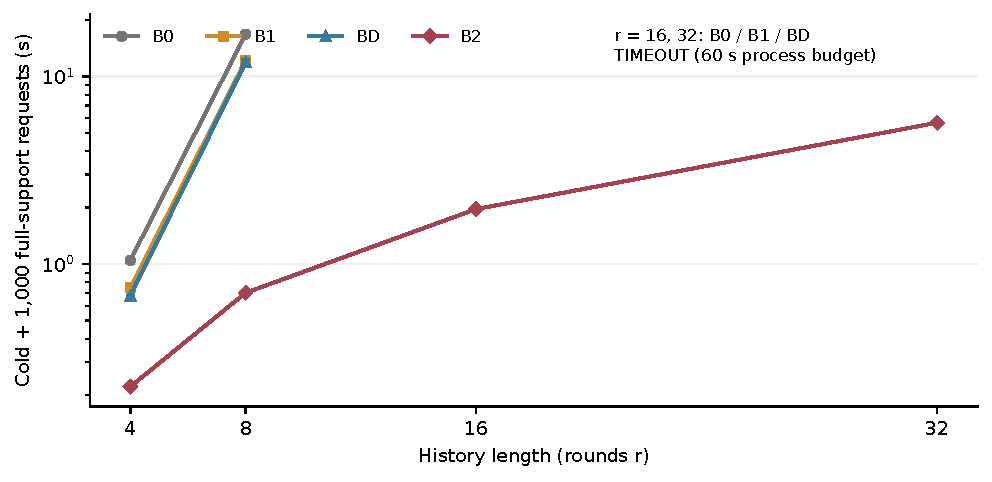
\includegraphics[width=.96\linewidth]{figures/history_cost.pdf}
\caption{分支缓冲固定 $C=3$ 的历史增长。横轴为轮数 $r$，纵轴为冷启动加 $1000$ 次完整支持请求的秒数，对数刻度；成功点为三次重复的中位数及最小／最大范围。未完成点不作为成功曲线点。主缓冲扫描批次。}\label{fig:historycost}
\end{figure}

图~\ref{fig:historystates} 和表~\ref{tab:historystructure} 将关系压缩与输出规模分开。最大层状态 $S_{\max}$ 始终为 $30$，总状态和转移随历史有规律地增长；每轮仍增加真正有多个来源的读。与此同时，原始变量数从 $108$ 增至 $5680$。这些变量含退休事件及常量，完整支持服务必须继续回答它们。$32$ 轮的查询部分约为 $4.82$ 秒，超过约 $0.53$ 秒的图编译时间。恒定 $S_{\max}$ 因此不意味着恒定端到端时间或内存。成功工作进程的最大峰值约为 $691$ MiB，全部低于 $1$ GiB；六个超时点的进程树复核仍为时间超限，峰值为 $111$--$221$ MiB。

\begin{figure}[t]
\centering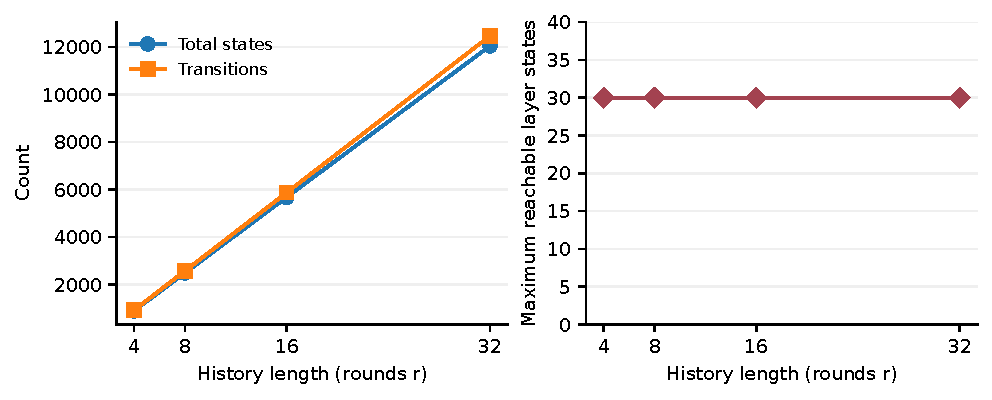
\includegraphics[width=.96\linewidth]{figures/history_states.pdf}
\caption{同一 $C=3$ 扫描的状态规模。左图为总状态／转移，右图为最大可达层状态；两者均为计数，各自使用独立纵轴。三次成功重复的结构统计一致。理论中的指数上界 $S_{\rm bd}$ 不在本图中充当预测值。}\label{fig:historystates}
\end{figure}
\begin{table}[t]
\centering\small
\caption{固定 $C=3$ 的缓冲结构。$n$ 包含初始化事件；$|D|$ 为剩余 RF 候选总数；所有输入的未决 CO 数均为零。}\label{tab:historystructure}
% Generated from frozen JSON; do not edit.
\begin{tabular}{rrrrrrrrrr}
\toprule
$r$ & $n$ & $|X|$ & $|D|$ & 歧义读 & $K$ & 组数 & $S_{\max}$ & 状态 & 转移 \\
\midrule
4 & 38 & 108 & 30 & 6 & 10 & 122 & 30 & 899 & 928 \\
8 & 70 & 388 & 66 & 14 & 12 & 234 & 30 & 2491 & 2576 \\
16 & 134 & 1464 & 138 & 30 & 12 & 458 & 30 & 5675 & 5872 \\
32 & 262 & 5680 & 282 & 62 & 12 & 906 & 30 & 12043 & 12464 \\
\bottomrule
\end{tabular}

\end{table}

这种压缩也不依赖把缓冲各阶段拆成互不关联的小问题。预处理后的 CNF 在每个主缓冲输入中都有一个包含全部未固定原始位的组件。连通性本身只描述公式表示；额外的原始语义核查给出真正跨阶段关联：在 $16$ 轮、$C=3$ 输入中，$\RF{W_8}{Q5\_peer}$ 与 $\RF{A_6}{P6\_peer}$ 分别可满足，但合取不可满足。它们分属第 $6$ 和第 $7$ 阶段，排除了这两个阶段选择完全独立的解释。$8$ 轮、$C=4$ 还具有第 $6$ 与第 $8$ 阶段的相应冲突。

\subsection{容量扩大与可达状态预算}\label{sec:capacityexp}
表~\ref{tab:capacity} 固定 $r=8$ 改变容量。$C$ 从 $3$ 到 $4$ 时，$K$ 从 $12$ 增至 $15$，而 $S_{\max}$ 从 $30$ 增至 $294$，状态总数增长明显快于处理组数。B2 仍可完成，但构造和千次支持查询的总时间增至约 $4.21$ 秒。这说明容量窗口会实质影响联合状态，不只增加若干事件。

\begin{table}[t]
\centering\small
\begin{threeparttable}
\caption{固定 $r=8$ 的容量扫描。时间为冷启动加 $1000$ 次完整支持请求的秒数，成功点取三次中位数。}\label{tab:capacity}
% Generated from frozen JSON; do not edit.
\begin{tabular}{rrrrrrrr}
\toprule
$C$ & $\max|D(r)|$ & $K$ & 组数 & $S_{\max}$ & 状态 & BD (s) & B2 (s) \\
\midrule
2 & 2 & 9 & 219 & 4 & 501 & 3.6265 & 0.2857 \\
3 & 3 & 12 & 234 & 30 & 2491 & 11.8927 & 0.7028 \\
4 & 4 & 15 & 247 & 294 & 16819 & 22.8425 & 4.2130 \\
6 & 6 & 17 & 267 & $\ge 12420$\tnote{a} & 200001\tnote{a} & 38.2462 & 状态上限 \\
\bottomrule
\end{tabular}

\begin{tablenotes}[flushleft]\footnotesize
\item[a] $C=6$ 在第 $187$ 个处理步骤触发状态预算；所列状态是失败时的部分计数，$S_{\max}$ 仅为完整构造的下界。\texttt{STATE\_LIMIT} 表示没有进入查询。
\end{tablenotes}
\end{threeparttable}
\end{table}

$C=6$ 在约 $28.38$ 秒触及状态预算，此时已产生 $200\,001$ 个状态和 $205\,322$ 条转移。B0、B1、BD 则均完成，分别约为 $47.41$、$37.49$ 和 $38.25$ 秒。因此当前实现的正面区间是已测的 $C=2,3,4$；$C=6$ 给出明确的工程边界。没有测量的 $C=5$ 不能被当作已经定位的阈值，状态预算失败也不意味着扩大预算后一定无法构造。容量、候选域、$K$ 和可达状态同时变化，测量支持整体机制解释，不把全部耗时差异归给单一结构参数。

为检查对请求池的敏感性，另在 $r=8,C=3$、$r=4,C=3$ 和 $r=8,C=4$ 各使用两个新池，每池测试原顺序和固定洗牌，每个设置两次重复。四组池／顺序的 B2/BD 总时间比分别处于 $0.055$--$0.064$、$0.284$--$0.321$、$0.178$--$0.185$，优势方向未改变。这只覆盖既定的假设长度及 SAT 比例分布。$r=4,C=3$ 是成功点中比值最接近 $1$ 的点，但仍明显有利于 B2，不是一个实测收益交叉点。

\subsection{新假设、局部复用和布局的解释}\label{sec:reuseexp}
图~\ref{fig:reuse} 使用独立的屏障查询复用批次，固定 $Q=1000$，令不同全局假设数 $U$ 为 $21,100,500,1000$。$U=21$ 时共有 $979$ 次全局答案命中；$U=1000$ 时全部请求都是新条件。随着全局复用降低，B1 成本显著增加，B2 的图扫描成本也增加。BD 却能继续复用局部结果，并在全部新条件时优于 B2。

\begin{figure}[t]
\centering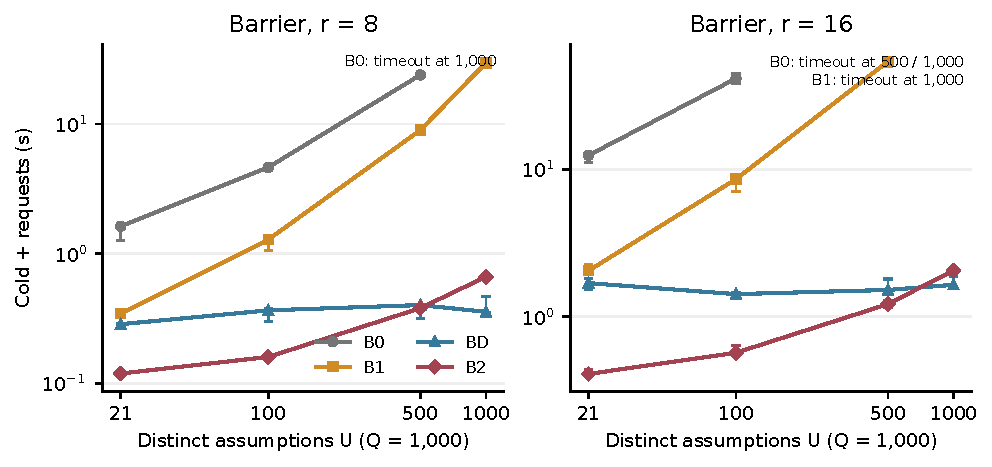
\includegraphics[width=.96\linewidth]{figures/query_reuse.pdf}
\caption{屏障上全局新假设数量与成本。$Q=1000$，横轴为不同假设数 $U$；纵轴为冷启动加请求成本，秒，对数刻度。成功点三次重复，中位数及最小／最大范围；标注的超时点没有绘制虚构耗时。该图来自查询复用批次，独立于图~\ref{fig:historycost} 的主缓冲扫描。}\label{fig:reuse}
\end{figure}

原因可以直接核查。在可穷举的 $1,2,3$ 轮上，完整关系分别有 $9,81,729$ 个模型，并等于按工作区分解后的直积，跨轮原始位固定。在实际 $8,16$ 轮残余 CNF 中，自动组件提取分别得到 $8,16$ 个含原始自由位的组件，每个有 $6$ 个原始自由位和 $9$ 个局部模型。BD 不需要知道轮号便可以利用这一结构。当 $U=1000$ 时，$8,16$ 轮 BD 只有 $82,154$ 次局部缓存缺失，尽管全局缺失各为 $1000$。表~\ref{tab:reuse} 给出这些请求及答案数量。所测屏障的恒定层状态并不能证明持续的跨轮关联；缓冲的语义反例承担了后一项证据。

\begin{table}[t]
\centering\small
\caption{屏障查询复用的解释量。不同完整答案数包含统一的不可满足答案；时间为三次中位数。局部缺失统计来自 BD 自动提取的 CNF 组件。}\label{tab:reuse}
% Generated from frozen JSON; do not edit.
\begin{tabular}{rrrrrrrr}
\toprule
$r$ & $U$ & 全局命中 & 不同答案 & BD 局部缺失 & B1 (s) & BD (s) & B2 (s) \\
\midrule
8 & 21 & 979 & 12 & 51 & 0.3451 & 0.2854 & 0.1188 \\
8 & 100 & 900 & 91 & 82 & 1.2814 & 0.3647 & 0.1594 \\
8 & 500 & 500 & 491 & 82 & 8.9654 & 0.4008 & 0.3793 \\
8 & 1000 & 0 & 991 & 82 & 29.6376 & 0.3552 & 0.6621 \\
16 & 21 & 979 & 12 & 66 & 2.0491 & 1.6897 & 0.4088 \\
16 & 100 & 900 & 91 & 150 & 8.5698 & 1.4225 & 0.5693 \\
16 & 500 & 500 & 491 & 154 & 53.9582 & 1.5183 & 1.2179 \\
16 & 1000 & 0 & 991 & 154 & 超时 & 1.6464 & 2.0603 \\
\bottomrule
\end{tabular}

\end{table}

布局消融也显示宽度界与实测成本的区别。$16$ 轮屏障的稀疏 CO 表示为 $K=13$，冷启动加 $100$ 次查询约 $0.516$ 秒；稠密 CO 为 $K=162$，约 $2.878$ 秒。但稠密化还增加了处理组和状态数，不能把约 $5.6$ 倍差异全部解释为 $K$ 的单独作用。普通输入布局取 $K=15$，约 $0.493$ 秒，反而略快于专用布局。长写间隔变体中，专用／普通布局在 $16$ 轮分别为 $K=15/17$、约 $0.525/0.489$ 秒。附录表~\ref{tab:mechanism} 同时列出组、状态、转移及计划、编译、查询分项。理论贡献是一个有证明且无需搜索的构造，实际耗时还由可达状态、处理组数和计划费用决定。

\subsection{按需诊断中的收益反转}\label{sec:diagnosis}
我们把第~\ref{sec:queries}节的日志编辑任务应用于 $8$ 轮屏障与 $8$ 轮、$C=3$ 缓冲。每份输入含 $32$ 段日志，其中 $16$ 段具有跨字段冲突，$16$ 段为对应一致记录。客户端加入字段、求删除极小冲突、枚举全部单字段修复、选择确定排序的首个修复，再撤销和恢复一个字段。四种方法得到相同冲突、修复集合与支持快照；屏障共有 $32$ 个替代修复，缓冲共有 $46$ 个。

两种输出模式改变任务需求。最终快照模式只在每段末尾输出一次完整支持，共 $32$ 次；频繁快照模式还在一致编辑后输出，共 $128$ 次。两者均另有 $208$ 次一致性请求和 $32$ 次字段支持请求。B0/B1 的删除检查只问 SAT，修复只求目标字段；BD 限定到相关组件，B2 用可达性做一致性。相同的是请求及其结果，不要求相同内部 SAT 调用次数。

\begin{figure}[t]
\centering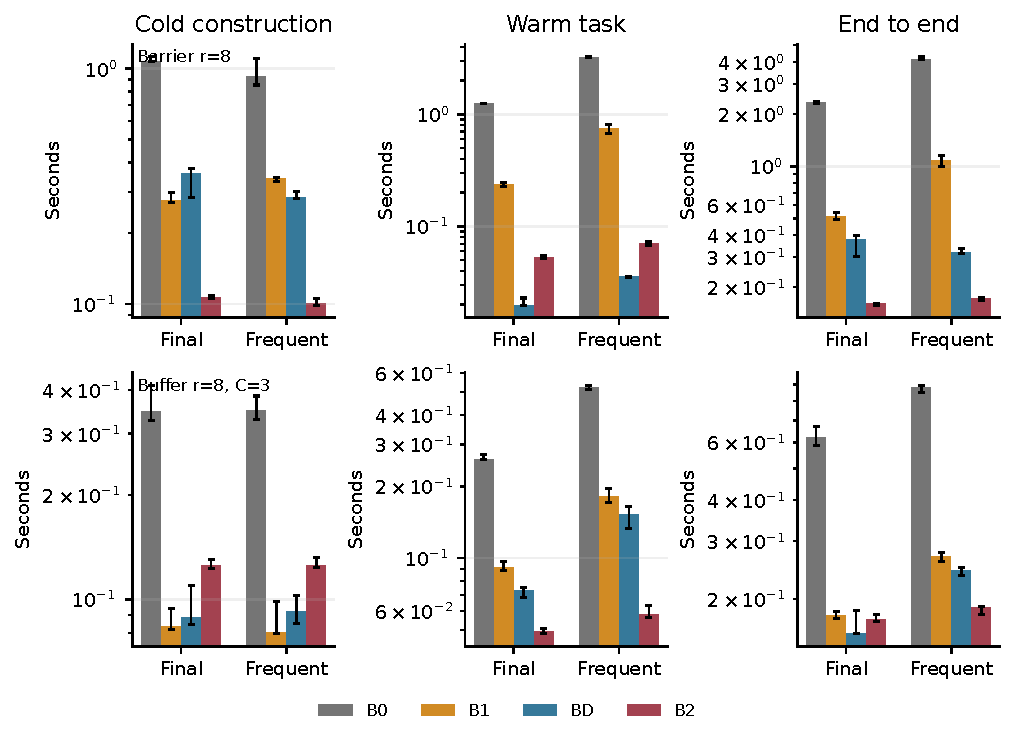
\includegraphics[width=\linewidth]{figures/diagnosis.pdf}
\caption{相同日志诊断任务的冷启动、温态与端到端成本，单位秒，均为对数刻度。Final 为最终快照，Frequent 为频繁快照；每点三次进程重复，柱为中位数，误差线为最小／最大范围。三个分项独立统计并分图绘制，没有把独立中位数强行堆叠。诊断批次包含结果序列化费用。}\label{fig:diagnosis}
\end{figure}

图~\ref{fig:diagnosis} 显示任务结构可以改变方法排名。缓冲最终快照模式中，BD 为 \BufferSparseBD\ 秒，B2 为 \BufferSparseBTwo\ 秒；温态查询收益不足以覆盖 B2 更高的冷启动成本。频繁快照模式中，BD 为 \BufferDenseBD\ 秒，B2 为 \BufferDenseBTwo\ 秒，B2 才取得端到端优势。其幅度约为 $1.30$ 倍，显著小于主接口实验千次新完整支持请求的约 \BufferRatio\ 倍。两种请求结构不能互换加速比。

屏障又体现另一种成本来源。BD 的最终／频繁快照温态约为 $0.0198/0.0354$ 秒，快于 B2 的 $0.0524/0.0700$ 秒；B2 的端到端领先伴随更低构造成本。结果支持按任务需求选择复用方式：同一套精确支持表示可以服务多种请求，但完整编译的投入是否值得，要连同冷启动、局部缓存及完整快照频率一起判断。

\subsection{正确性证据与适用边界}
小实例检查直接比较完整原始赋值集合：对 $36$ 个可枚举案例分别枚举 RF 与逐地址 CO，与接受路径投影双向核对；另对极小输入穷举 $1152$ 个布尔原始赋值，包含违反恰一 RF 或总 CO 的非法赋值。查询核对覆盖条件冲突、撤销、已退休事件和固定原始位。单轮屏障工作区的 $9$ 个模型中有 $2$ 个 RF／CO 赋值没有 SC 线性化，这没有把整个读值观测误称为 SC 不可达。

较大输入采用不读取 $D/H/L$ 的原始 RA SAT 编码，核查 $494$ 个预先选定的排除：$168$ 个永久删除 RF、$168$ 个固定 CO 的反向、$158$ 个条件下不支持文字，全部不可满足，无未知结果。条件样本中 $134$ 个来自缓冲跨阶段关联，$24$ 个来自屏障局部关联。对条件本身和撤销条件后恢复的目标文字做正对照，加上根输入共 $323$ 次可满足检查；所获完整赋值再按独立的稠密 $\hb/\eco$ 定义验证。样本覆盖容量边界、模数回绕、失败尝试、失败尾链和未完成调用。这里独立的是原始语义编码相对于协议过滤及编译图；没有第二套 SAT 求解器或 DRAT/LRAT 证明日志。$32$ 轮输入只在已完成基线的公共请求前缀上比较完整答案，不能把 B2 的全部千次结果称为已获原始 SAT 全量确认。

这些实例是来自明确协议结构的生成观测，尚无工业日志覆盖率调查。更早的重复发布内核还保留了恒定载荷六轮构造超预算、四轮按需 SAT 更快的结果；改用轮次版本值会缩小来源域，这部分收益来自观测信息增加。第一轮屏障测量中，温态 SAT 和单文字查询也快于完整支持扫描。这些结果共同限定性能主张：协议界说明存在可控的候选接口，具体收益仍取决于可达状态、可提取分解、输出规模和请求类型。BD 只是静态组件基线；没有同投影任务上的成熟编译器对照，实验不支持胜过通用知识编译工具的结论。

\section{相关工作}\label{sec:related}
协议逻辑已经说明，读取共享状态能够获得关于协议进展的知识。GPS 使用单地址协议、幽灵状态与资源转移推理弱内存程序，并以循环缓冲展示资源复用~\cite{gps2014}；iGPS 的读规则允许从当前已知协议状态前进到某个后继状态，单写者协议进一步支持常见更新纪律~\cite{igps2017}。因此“同步能传递不可逆知识”是本文的推理基础。本文进一步研究这种共同知识对\emph{所有尚未选择的候选}产生什么图结构限制：在候选过滤饱和后，稳定历史只保留每地址的少量极大写，再连接完整原始支持。缓冲窗口来自双向反馈；屏障的来源下界还利用了到达位的真实重置，不依赖完整交替日志的末端计数。

内存关系分析为候选与必然事实提供了成熟抽象。Haas 等人的 may/must 过滤框架允许程序信息、关系方程与模型公理双向传播~\cite{haas2023}。其具体过滤语义定理与可靠抽象过滤需要区分：可靠简化保留合法执行，但近似域本身并不等于精确支持。本文的 $R_\forall$ 可以作为这类分析中的具体规则；新结构结论需要额外证明 R1/R2 饱和、稳定极大写及 RF／未决 CO／覆盖边的共同边界，而不能从 may/must 可靠性直接读出 $K$ 的参数界。CAAT 将一致性作为可用于 SMT 的理论，并研究关系固定点计算和冲突解释~\cite{haas2022}。其 §4.1 讨论删除边后复用固定点的困难。本文通过预编译固定输入，对路径标签条件化来支持撤销；这里撤销的是原始假设，事件结构保持固定。

给定 RF 后补全修改序，与同时保留所有 RF／CO 选择是相关但不同的任务。Tunç 等人的 reads-from consistency checking 接收事件、程序顺序和已经选择的 RF，检查是否存在合法修改序，并对多种 C11 风格模型给出高效算法~\cite{tunc2023}。这项工作已经处理未知 CO。本文需要将不同 RF 选择共同保留，并回答任意附加 CO 条件后的全部支持，因此最终表示不能把 CO 仅作为无须查询的存在见证消去。

Conrado 与 Pavlogiannis 的 MSO 框架研究已选 RF 图的结构和弱内存可定义性~\cite{conrado2026}。其 Lemma~1 约束 SC 的 RF 图树宽，Lemma~4 把高树宽联系到任意 $\SB\cup\rf$ 拓扑序中的大写距离；文中也明确展示长 RF 边可以与低树宽并存。其 Theorem~9 和 Lemma~10 给出 RA 等模型在 RF 图上的 MSO 表达，结合结构结果得到验证与 RF 鲁棒性算法。本文控制的对象还包括全部 RF 候选、未决 CO 与固定 CO 覆盖边，所用布局先于所有完成确定。第~\ref{sec:frontier}节的 $K_{h,h}$ 例子说明为何逐完成结构界不能直接推出这一结论。稳定写代表进一步把共同因果关系转为可构造的候选接口界；长边存在但端点少这一观察本身不是贡献边界。

复杂度结果解释了为何还需要协议条件。Chakraborty 等人证明，RA 及其相关变体的一致性测试即使在线程数、地址数和值域有界且没有 RMW 时，仍为 NP 完全~\cite{chakraborty2024}。Govind 等人进一步研究每地址写者数：单写者的 RA／SRA／WRA 一致性测试可多项式求解，而允许两个写者时已有 NP 完全性~\cite{govind2026}。这些结论针对各自的观测测试问题，不直接成为本文协议子类的下界。特别是单写者缓冲的实验价值在于重复条件支持及实际跨阶段关联，不能表述成把一个已知困难的单次判定问题变为易解。多写者屏障则说明前沿参数可以在写者数大于一时仍然受控。

关系自动机与知识编译提供后端基础。Kater 用关系代数、自动机及闭合游走检查处理内存模型元理论和一致性~\cite{kater2023}；本文沿用正则关系监视的思路。路径表示上的条件化、投影与查询能力属于知识编译的标准研究对象~\cite{darwiche2002}，由平滑 DNNF 构造支持传播编码也已有系统结果~\cite{kucera2021}。本文特别保持原始变量投影，使用同一历史的普通／一标记摘要建立可接受后缀等价，再保留路径标签。通用编译步骤不是单独的创新主张。d4 等编译器已经利用动态分解和组件缓存~\cite{lagniez2017}；本文静态 BD 对照用于识别局部分解对收益的解释范围，没有与这些成熟编译器在相同任务上作性能排名。

\section{结论}
同步协议决定可以安全遗忘多少历史，关键在于历史事件与未来相关访问之间已经共同确定的因果关系。本文证明：未决因果前沿之外，仍需连接未来的稳定写可以由每地址至多一个线程数规模的极大集合表示；这同时控制 RF 候选、未决 CO 和固定 CO 覆盖边。反馈缓冲与重置／唤醒屏障提供了从实际协议纪律构造这种结构的两条路径，原始身份则由精确编译的路径标签保留。

冻结实验显示，固定容量缓冲的历史增长可以保持小的可达层状态，而扩大容量、降低全局复用或改变快照需求会改变构造可行性与方法排名。因果前沿因而给出一个可证明的结构保证，精确投影把它用于反复查询，实际任务的复用和输出需求决定这项编译投入何时值得。

\bibliographystyle{plainnat}
\bibliography{references}
\clearpage
\appendix
\section{结构与协议证明的补充细节}\label{app:protocols}
\subsection{原子来源组的附加参数}\label{app:atomic}
第~\ref{sec:frontier}节的二元候选边界不能直接覆盖原子 RF 超边。若另有 $d=\max_r|D(r)|$，把每个原子组 $\{r\}\cup D(r)$ 安排在其最晚端点引入时处理，所有端点连续保留到该位置。考虑切口处一个因该超边而额外存活、却没有二元未来邻居的旧写 $w$。组中心读 $r$ 必在过去，否则 $w$ 就有未来邻居 $r$；该组又必有某个未来候选写 $v$。由 R1 饱和，$v\in D(r)$ 意味着 $\neg H(r,v)$，所以 $r\in U_t$。每个这样的读最多贡献 $d$ 个额外旧写。因此在定理~\ref{thm:frontier} 的袋上增加至多 $cd$ 个端点，即得
\[
 K_{\rm atomic}\le c(d+1)+ap+p+a+1.
\]
按最后端点调度且一直保留端点保证超边覆盖和连续生存期。这个结论以 $d$ 为附加参数；若它随历史增长，则不能得到仅依赖 $c,p,a$ 的统一常数界。

\subsection{无界纯失败读链的完整袋展开}\label{app:chains}
对第~\ref{sec:buffer}节程序，识别由已观测失败分支确定的极大连续失败尝试串。串内每次尝试只有两个索引读，没有载荷事件、写或其他地址访问。引理~\ref{lem:bufferwindow} 及自身索引唯一性给出阶段 $k$ 的固定来源锚：生产者失败串使用 $W_{k-1}$ 与 $A_{k-1-C}$，消费者失败串使用 $W_{k-1}$ 与 $A_{k-1}$。负下标对应的失败分支已被证明不可能；初始化锚另计。

规划骨架保留全部成功操作和每线程最后尚未决定分支的调用，每骨架阶段最多 $b_0=2(B+3)$ 个事件。骨架只用于安排袋；所有 $H/L$ 和来源域仍从完整原始输入证明得到。暂时缩去失败链，不等于删除输入事件后重新解释一个协议。特别是被缩去的链首尾所形成的规划连接不作为额外 $\SB$ 语义边加入后端。

为每串登记来源锚及左右真实线程端点，在其所属阶段 $k$ 设置处理位置。把已引入的阶段 $[k-C-1,k]$ 骨架事件连续保留到该位置及阶段末尾。该窗口有 $C+2$ 个阶段，所有非初始化锚和左右端点都位于其中；左端点属于阶段 $k-1$ 或 $k$，右端点若存在则属于 $k$。若完整输入以纯失败串结束而该阶段没有骨架事件，则增加一个仅用于计划的虚拟处理位置，缺失右端点不补造。

对于窗口之前仍有实际候选连接的骨架事件，采用定理~\ref{thm:frontier} 的逐边论证。阶段分隔使旧读不再具有未来 RF，旧写与未来写的未决 CO 不存在；若旧稳定写不为稳定极大写，R2 删除其未来 RF，且中间稳定写阻止它成为 CO 覆盖前驱。它们至多贡献 $ap$ 个写。骨架线程连接另需至多 $p$ 个尾端点，初始化需 $a$ 个。实际候选边界及登记位置决定生存期；稳定极大集合只用于计数，不能让已经退休事件因后来成为极大元素而重新出现。因此所有锚同时可用时，骨架袋大小至多
\[
 (C+2)b_0+ap+p+a.
\]

在该袋处一次展开一条串：引入第一个真实读，加入其固定 RF 及左侧真实线程边；逐个引入下一读，处理它的固定 RF 和前一读到它的线程边，再退休前一读；最后处理末读到右端点的边。最多同时增加两个读。原袋端点在整个展开期间连续保留，新读也只在连续区间出现；不同串顺次展开。于是 $K\le(C+2)b_0+ap+p+a+2$，代入 $p=2$ 得式~\eqref{eq:chainbound}。

骨架袋允许右线程端点先于中间读引入。这是图处理顺序，真正加入语义的仍只有每条原始邻接边与所有真实读。读的固定正 RF 以及所有被排除候选的负 RF 保留唯一标签归属；监视器仍经过这些读计算 HB、FR 和禁止游走。因此展开保持完整投影，而不是只保持删除失败读后的一个商输入。若重试体还含其他工作，这个纯链证明不适用，应在阶段工作量参数中计入那些事件。

\subsection{屏障失败等待和未完成前缀}\label{app:barriertails}
引理~\ref{lem:barrier} 的成功对齐还确定到达地址的 CO。$A_{t,i}\mathrel\rf R_{t,i}\mathrel\SB Z_{t,i}$ 给出 $A_{t,i}<_{\co}Z_{t,i}$；$Z_{t,i}\mathrel\SB G_{t,i}\mathrel\rf S_{t,i}\mathrel\SB A_{t,i+1}$ 给出 $Z_{t,i}<_{\co}A_{t,i+1}$。初始化最小，形成正文所列交错写链，截断前缀只会删除末尾而不会插入未观测事件。

证明正文布局中失败读不属于前沿，需要分别检查两类等待。协调者调用 $i$ 中对 $a_t$ 的失败读 $f$，若本轮到达写 $A_{t,i}$ 存在，已经在布局的工作者步骤引入。本轮及以后重置 $Z$ 在线程中都位于 $f$ 之后。未来工作者到达 $A_{t,j}$、$j>i$ 若存在，则其前缀和成功对齐要求 $S_{t,i}$ 存在，并给出
\[
 f\mathrel{\SB^+}G_{t,i}\mathrel\rf S_{t,i}\mathrel{\SB^+}A_{t,j}.
\]
若当前等待未成功且所需到达事件缺失，合法前缀就不能含需要它的后续唤醒及更晚调用。这不是根据调度假定其发生，而是由非空成功来源域导出的必要存在性。因此所有仍在未来的同地址写均在 $H(f,\cdot)$ 后方。

工作者调用 $i$ 的失败唤醒读 $f$ 访问 $g_t$。本轮 $G_{t,i}$ 若存在，已在协调者步骤引入；未来只能有 $G_{t,j}$、$j>i$。其存在要求 $R_{t,j}$ 及准确来源 $A_{t,j}$ 存在，因此
\[
 f\mathrel{\SB^+}A_{t,j}\mathrel\rf R_{t,j}\mathrel{\SB^+}G_{t,j}.
\]
这说明 $f$ 对所有未来同地址写稳定。若不存在未来写，稳定条件自然成立。读与未来同地址读不构成式~\eqref{eq:frontier} 中的相关对。于是全部失败读均被排除出 $U_t$，它们的线程边仍由通用界的尾事件项处理。

任意阶段 $i$ 的工作者事件在其下一到达 $A_{t,i+1}$ 之前；下一到达通过成功读取进入协调者，再经其全部到达之后的唤醒进入任意线程的阶段 $i+2$。协调者阶段 $i$ 的事件直接沿程序顺序到下一轮唤醒。只要目标阶段 $i+2$ 的事件存在，所有这些必要交接都由前缀和成功对齐强制存在。因此阶段差至少二的事件均有共同 $H$。去掉已证明稳定的失败读，切口最多剩两个阶段各 $b_0$ 个骨架事件，得到式~\eqref{eq:barrierbound}。

\subsection{地址封闭组合的证明}\label{app:composition}
设地址分区为 $\mathcal A_1,\ldots,\mathcal A_h$，$E_i$ 包含访问 $\mathcal A_i$ 的全部事件及相应初始化。局部线程顺序是全局线程序在 $E_i$ 上的限制；它的邻接边可以跨过其他组件的事件。局部协议元数据必须与这个控制投影兼容；观测约束采用由全局输入蕴含的局部限制。

任取全局合法完成 $J$。局部读的真实来源因为同地址闭合仍在 $E_i$ 内，局部 CO 是原地址的完整写序；局部线程边对应全局线程路径，所以局部 $\hb$ 包含于全局 $\hb$。局部 $\eco$ 也包含于全局 $\eco$。若局部出现禁止闭环，全局也出现同一闭环，矛盾。因此 $J|E_i$ 合法，局部已证 $H_i$ 在全局中可靠。将全部 $H_i$ 与全局 $\SB$、初始化取传递闭包，仍为所有全局完成的共同下界。

建立布局约束图 $T$，加入每个局部总排列 $\theta_i$ 的邻接边及全局线程邻接。若 $T$ 无环，固定一个拓扑序 $\theta$。由于每个 $\theta_i$ 为总序，$\theta$ 在 $E_i$ 上的投影恰为 $\theta_i$；全局每个切口对应局部的某个切口。取 $e\in U_t$ 及其未来相关见证 $f$，二者因同地址而属于同一个 $E_i$。若 $e\notin U_i$，局部稳定性给出 $H_i(e,f)$，进而给出全局 $H(e,f)$，与 $e\in U_t$ 矛盾。所以 $U_t\subseteq\bigcup_i U_i$，得到 $c\le\sum_i c_i$ 和正文组合界。

地址闭合不可省略。若把两个各自只写同一个 $x$ 的线程分成两个“组件”，每个局部前沿均为零；全局却有未决 CO 的完全二部候选，前沿可随写数增长。相容性也不可省略：局部总排列与跨组件线程边可能有环，表示给定计划无法合并，不能由此判断 RA 观测无解。对于无界失败缓冲，式~\eqref{eq:chainbound} 只给袋大小而非原始前沿界，故不能把该 $K$ 当作局部 $c_i$ 代入组合定理。可直接组合的是实际已给 $\SB$ 相容布局和前沿界的局部组件。

\subsection{完整交替发布网络的无写覆盖推论}\label{app:publication}
为明确第~\ref{sec:frontier}节的推论范围，设 $p$ 个线程构成直径为 $d$ 的固定强连通有向网络。每线程独占一个初值 $0$ 的标志；共有同样的 $h_0$ 个完整阶段，阶段 $i$ 向本线程标志写至少两次相同值 $i\bmod2$，再对每条入边读对方标志，观测 $(i-1)\bmod2$。这些是标志的全部访问，标志与数据地址分离，每阶段全部线程事件数至多 $b$。

对一条网络边，接收线程的 $h_0$ 个读按程序顺序排列。单写者 CO 和 RR 一致性使来源块号非降；交替读值使块号严格增加。最后一个读的值与最后一个写块不同，因此其块号至多 $h_0-1$。$h_0$ 个非负严格递增块号只能为 $0,1,\ldots,h_0-1$，其中 $0$ 是初始化。故第 $i$ 次等待的来源锁在对方第 $i-1$ 块，但块内身份仍可歧义。第一次发布是该块全部候选的共同前序，使用 $R_\forall$ 即得共同交接。

线程 $t$ 阶段 $i$ 的任意事件先于它阶段 $i+1$ 的首次发布，该发布又先于邻居阶段 $i+2$ 的对应等待。沿长度至多 $d$ 的网络路径重复这一步，再到目的线程下一阶段，可得阶段差至少 $2d+1$ 的共同因果分隔。因此 $c\le(2d+1)b$，无需规定数据地址的写频率。

这一改进有具体的参数分离族。在正文两线程发布内核中增加地址 $z$：A 只在第一阶段写 $z=1$，中间每阶段读 $z=1$，最后阶段再写 $z=1$。$p,a,b,d$ 均可固定，而最长无写区间随阶段数增加。两个非初始化写形成一条跨越整个历史的 CO 覆盖边，所有中间读仍来自首写；它们本就在同一线程顺序中，因而不为旧事件增加跨线程 HB，且自身一致性直接成立。一个稳定旧写可以承载这些长边。这里分离的是统一参数界，不声称每个有限输入都不能选取某个随规模增长的有限写覆盖参数。

\subsection{同值发布例子的完整见证}\label{app:witness}
为第~\ref{sec:example}节补齐省略事件。$x,y,fa,fb$ 初始化均为 $0$。对 $i=1,2$，两个线程依次执行
\begin{align*}
 A_i:\ &A_i{:}x=\W(x,1);\ A_i{:}0=\W(fa,i\bmod2);\ A_i{:}y=\W(y,1);\\
        &A_i{:}1=\W(fa,i\bmod2);\ A_i{:}w=\R(fb,(i-1)\bmod2);\ A_i{:}r=\R(x,1),\\
 B_i:\ &B_i{:}y=\W(y,1);\ B_i{:}0=\W(fb,i\bmod2);\ B_i{:}x=\W(x,1);\\
        &B_i{:}1=\W(fb,i\bmod2);\ B_i{:}w=\R(fa,(i-1)\bmod2);\ B_i{:}r=\R(y,1).
\end{align*}
正文的 $a_0,u,a_1,v,r,s$ 分别为 $A_1{:}0,A_1{:}y,A_1{:}1,B_2{:}y,B_2{:}w,B_2{:}r$。所有数据读选择本线程本轮的首个数据写，第一轮两个等待均选择初始化。反向 CO 见证取第二轮等待都读对方第一轮早发布，并取
\begin{align*}
 x:&\quad i_x<B_1{:}x<B_2{:}x<A_1{:}x<A_2{:}x,\\
 y:&\quad i_y<B_1{:}y<B_2{:}y<A_1{:}y<A_2{:}y.
\end{align*}
标志 CO 为初始化之后按各自线程顺序。它满足 $d\land e\land\neg q$。所有跨线程非初始化 RF 只到第二轮的末尾等待；因此 HB 无环。对于数据地址，来自对方早发布之前的数据写只能到达另一个地址的数据读：$A_1{:}x$ 到 $B_2{:}r$，$B_1{:}y$ 到 $A_2{:}r$。不存在与反向 CO 冲突的同地址跨线程 HB。各线程内部的同地址来源与写序依次前进，满足 WW／WR／RW／RR。标志读选择的早发布之前没有更晚同地址 HB 前驱写，其未来同地址写在后续块；同样满足四类一致性。因此完整赋值合法。

正向见证把 $x,y$ 的 CO 都按轮拼接，轮内两写任意选择；第二轮等待可选择对方第一轮的早或晚发布。所有跨线程 HB 严格增轮，同轮仅有线程内部 HB，来源为本线程本轮写。由此 WW 与轮序相容，WR 的同轮同地址前驱至多为实际来源，RW 的后继写在以后轮，RR 来源轮号非降；标志按块顺序一致。分别选择 B 的早或晚来源，得到 $d\land e\land q$ 及 $d\land l\land q$ 的完整合法完成。正文对 $d\land l\land\neg q$ 的 WR 反证排除了最后一种组合。

\section{后端关系、支持编码与构造费用}
\subsection{四状态监视器的完整定义}\label{app:automaton}
式~\eqref{eq:language} 的部分 DFA 状态为 $0,1,2,3$，初态为 $0$，接受态为 $1,2$。非空转移如下，未列转移均不存在：
\begin{align*}
 s:&\quad 0\to1,\ 1\to1,\\
 r:&\quad 0\to1,\ 1\to1,\ 2\to2,\\
 g:&\quad 1\to2,\ 2\to2,\ 3\to2,\\
 \bar r:&\quad 1\to3,\ 2\to3.
\end{align*}
状态 $1$ 记录已经读过非空 $s/r$ 前缀，仍可延长该前缀；读到 $g$ 后进入只能读一致性后缀的状态 $2$；$\bar r$ 进入状态 $3$ 并强制随后至少一个 $g$。后缀中的 $r$ 可以继续停留状态 $1$，因为下一条 $s$ 仍可归入更长的因果前缀；一旦出现 $g$ 或完成 $\bar r g^+$，就不能再读 $s$。由此该 DFA 恰识别式~\eqref{eq:language}。

对每个事件 $e$，安装标记 $(e,1)\to(e,0)$ 和 $(e,2)\to(e,0)$。若事件图存在接受语言中的闭合游走，从 $(e,0)$ 沿乘积普通边到 $(e,1)$ 或 $(e,2)$，接一条标记便闭合。反之，任何恰一标记闭合游走可以旋转到该标记之后开始，其余全部普通边给出从初态到接受态、起止事件相同的游走。故二者等价。CO 监视器只有一个状态，每条 $g$ 边原样加入并要求普通图无环。

必须计数恰好一个标记。例如普通边 $0\to3,2\to1$，标记边 $1\to0,3\to2$ 形成两标记环，却没有恰一标记闭合游走。把普通边与标记边混合取闭包，或者允许 $T;T$，会错误拒绝这个关系状态。

\subsection{增量更新及端口投影}\label{app:update}
以下 $P$ 含普通恒等路径，$T$ 恰含一标记路径。插入普通边 $u\to v$ 前，若 $T(v,u)$ 则出现一标记环，应拒绝；否则用插入前的关系计算
\begin{align}
 P'&=P\cup P(*,u)\times P(v,*),\label{eq:updateP}\\
 T'&=T\cup T(*,u)\times P(v,*)\cup P(*,u)\times T(v,*).\label{eq:updateT}
\end{align}
普通路径中的新边若重复出现，可删去其间普通回路而不改变可达性。恰一标记路径若两次使用新边且标记处于其间，则存在旧 $T(v,u)$，已被拒绝；否则重复普通回路同样可去。于是列出的两类含标记扩展已经穷尽。

插入标记 $u\to v$ 前，若 $P(v,u)$ 则拒绝；否则
\[
 T'=T\cup P(*,u)\times P(v,*),\qquad P'=P.
\]
新标记不能与旧 $T$ 路径串接。CO 单状态图插普通边时检查 $P(v,u)$，随后使用式~\eqref{eq:updateP}。

每组完成后，投影到下一层由全部候选决定的 $I\times O$。装载下一层时恢复这些条目和普通恒等关系，再加入当前组新端点。可拼接的旧矩形条目仍在同一矩形中，其普通／一标记闭包已由前一层保存；未保留端点不可能再成为未来边的接口。引理~\ref{lem:ports} 的新旧段分解因此适用于投影后的更新。整个状态键还包括所有监视器和活跃读计数；逐监视器独立挑选代表历史不具有这个性质。

\subsection{支持 CNF 的完整构造}\label{app:supportcnf}
令接受 DAG 有唯一起点 $s_0$ 和终点 $t_0$，边 $e$ 的原始文字标签为 $\ell(e)$。固定文字可以作为公共起始边；每个原始变量在每条完整路径上恰被赋值一次。定义阻断条件
\[
 D_e=\bigvee_{\lambda\in\ell(e)}\neg\lambda.
\]
空标签使 $D_e$ 恒假。引入前缀不可达位 $A_v$ 与后缀不可达位 $Z_v$，按 DAG 顺序定义
\begin{align*}
 A_{s_0}&=\bot,& A_v&=\bigwedge_{e:u\to v}(A_u\lor D_e),\quad v\ne s_0,\\
 Z_{t_0}&=\bot,& Z_v&=\bigwedge_{e:v\to w}(D_e\lor Z_w),\quad v\ne t_0.
\end{align*}
空合取为真。对每个原始文字定义无支持位
\[
 W_\lambda=\bigwedge_{e:\lambda\in\ell(e)}(A_{\mathrm{src}(e)}\lor D_e\lor Z_{\mathrm{dst}(e)}).
\]
把这些无环电路以双向 Tseitin 子句编码，再加 $\neg Z_{s_0}$ 和每个 $W_\lambda\Rightarrow\neg\lambda$。常量的相反文字若没有任何边携带，其 $W$ 为空合取，会正确传播对应常量。电路和 CNF 大小均线性于图与标签出现次数。

在部分原始赋值 $\alpha$ 下，所有被阻断边的 $D_e$ 都由已知反文字传播为真。沿拓扑序归纳：若某节点无相容前缀，则所有入边要么被阻断，要么来自已传播不可达的前驱，故 $A_v$ 被传播为真。反向归纳得到所有无相容后缀的 $Z_v$。无接受路径时 $Z_{s_0}$ 为真，与单位子句冲突。若 $\lambda$ 不支持，任何携带它的边必在前缀、边阻断、后缀三种条件之一失败，因而 $W_\lambda$ 传播为真并推出 $\neg\lambda$。这个推导只用真的单调传播，不把未赋值文字当作假。

完整赋值 $x$ 若没有接受路径，会发生上述冲突；若有接受路径，则按电路的真实值赋辅助变量。任何 $x$ 为真的文字都在这条路径中出现，因此其 $W$ 为假，其余 $W_\lambda\Rightarrow\neg\lambda$ 也满足，得到 CNF 模型。这再次证明全赋值投影。由该精确投影，传播不会排除合法完成；支持不可能的反文字被排除，恰给出全部必然原始文字。该强度是相对原始变量的域一致性，与允许任意赋值辅助变量的传播完备性有区别~\cite{kucera2021}。

\subsection{协议构造的保守位复杂度}\label{app:complexity}
令 $L_{\rm in}$ 为包含事件、二进制值与容量、元数据和显式接口描述的输入位长度，$\ell=L_{\rm in}+|X|+1$。在二进制随机访问模型下，可用如下朴素实现得到 $O(\ell^8)$ 的预处理及复核上界，证书和完整计划编码长度为 $O(\ell^6)$。这是保守构造界，并非实验实现的实测增长拟合。

注册表枚举至多 $O(n^2)$ 个读写／写写对。两个协议的来源下界和候选上界只对显式事件实例化；每条候选可以列出至多 $n$ 个前提来源，代价至多 $O(n^3)$ 次关系或数值检查。一个容量值即使很大，算法也不遍历 $0,1,\ldots,C$；必要的数组地址及初始化必须已经显式列入输入。整数比较、加减及取模保守以两个 $O(\ell)$ 位整数的 $O(\ell^2)$ 位操作计费。

永久来源域只减，$H/L$ 只增，全部可能变化不超过 $O(n^2)$ 项。每次有变化的遍历用 $O(n^3)$ 次单元操作做闭包及全量 R1/R2/$R_\forall$ 检查，故饱和至多 $O(n^5)$ 次单元操作，连同数值和引用操作由 $O(\ell^7)$ 覆盖。地址闭合分区满足 $\sum_i|E_i|\le n$，局部及全局饱和总费用仍在同阶粗界中。覆盖边计算、前沿区间扫描、布局拓扑序、失败串登记和计划检查均为更低阶的显式多项式过程。

推导记录对每个永久事实只保存第一次理由，共 $O(n^2)$ 条。R1/R2 与闭包记录常数个先前事实，$R_\forall$ 最多列出 $n$ 个当前候选及共同前序；域用删除日志和版本标识重放，也可保守保存每轮矩阵快照。规范计划至多 $O(n^2)$ 层，每层列出至多 $n$ 个端点及归属引用，其长度为 $O(n^3\log(\ell+2))$。这些材料由 $O(\ell^6)$ 位覆盖；再独立重放记录及计划，保守 $O(\ell^8)$ 足够。复核检查的是已证明规则的有限前提，不调用“对所有完成成立”的语义 oracle。

接上式~\eqref{eq:size} 的后端，在固定协议参数 $\vartheta$ 下，只要相应协议界给出 $K\le g(\vartheta)$，总构造可写为 $f(\vartheta)\ell^{O(1)}$。参数分别包含缓冲的容量、地址数、工作量及在阶段版本中使用的失败次数界，或纯失败链版本的容量、地址数、工作量；屏障包含参与线程数、地址数、工作量；组合还包含组件数及每个实际前沿参数。这个结论不把协议识别、任意布局优化或未支持守卫的处理视为免费，也不把无界失败链的袋界代入需要原始前沿界的组合入口。

\subsection{原始 SAT 核对的投影理由}\label{app:oracle}
独立原始编码采用 RF 恰一、逐地址严格总 CO、输入守卫及一个辅助关系 $H_o$。令条件基本边 $B=\SB_{\rm adj}\cup\rf\cup\init$，加入 $B(u,v)\Rightarrow H_o(u,v)$、$H_o(u,v)\land B(v,w)\Rightarrow H_o(u,w)$ 及 $\neg H_o(u,u)$。同时用 WW／WR／RW／RR 子句约束 $H_o$ 与原始 RF／CO。它没有导入协议证书的来源删域或共同关系。

固定原始赋值后，按路径长度归纳有 $B^+\subseteq H_o$。四类一致性子句都以 $H_o$ 为前提，故把它缩小为 $B^+$ 不破坏子句；反自环保证实际 HB 无环，从而得到原始 RA 完成。反向，合法完成取 $H_o=B^+$ 就满足所有子句。因此编码的存在辅助变量投影是原始语义。这个证明解释了负支持核查为何不循环依赖待测证书；具体测量仍是选定样本的求解结果，不等同于对所有输入机械证明实现。

\section{补充结果与复现说明}\label{app:results}
表~\ref{tab:service} 补充主缓冲扫描的服务分项。冷启动包括证书生成及检查、编码或计划和编译。缺失计算为未命中完整答案缓存时的计算，输出列为形成完整支持列表的记录成本；各分项独立取中位数，且存在额外管理开销，所以不能将列相加作为总计。$C=2$ 有三次全局缓存命中，其余主点均无命中。

\begin{table}[p]
\centering\small
\caption{主缓冲扫描的服务成本细项，单位秒。$r/C$ 为轮数／容量，$U$ 为不同假设数，答案为不同完整支持答案数。成功点三次中位数；未完成不填最终请求统计。}\label{tab:service}
% Generated from frozen JSON; do not edit.
\begin{tabular}{llrrrrrr}
\toprule
$r/C$ & 方法 & $U$ & 答案 & 冷启动 & 缺失计算 & 输出 & 总计 \\
\midrule
4/3 & B0 & 1000 & 726 & 0.0462 & 0.9947 & 0.0043 & 1.0472 \\
4/3 & B1 & 1000 & 726 & 0.0218 & 0.7169 & 0.0037 & 0.7481 \\
4/3 & BD & 1000 & 726 & 0.0272 & 0.6446 & 0.0038 & 0.6771 \\
4/3 & B2 & 1000 & 726 & 0.0373 & 0.1769 & 0.0035 & 0.2223 \\
8/3 & B0 & 1000 & 991 & 0.3900 & 16.3947 & 0.0081 & 16.7957 \\
8/3 & B1 & 1000 & 991 & 0.0745 & 12.0800 & 0.0079 & 12.1646 \\
8/3 & BD & 1000 & 991 & 0.1009 & 11.7976 & 0.0088 & 11.8927 \\
8/3 & B2 & 1000 & 991 & 0.1238 & 0.5729 & 0.0059 & 0.7028 \\
16/3 & B0 & -- & -- & -- & -- & -- & 超时 \\
16/3 & B1 & -- & -- & -- & -- & -- & 超时 \\
16/3 & BD & -- & -- & -- & -- & -- & 超时 \\
16/3 & B2 & 1000 & 991 & 0.3290 & 1.5939 & 0.0197 & 1.9647 \\
32/3 & B0 & -- & -- & -- & -- & -- & 超时 \\
32/3 & B1 & -- & -- & -- & -- & -- & 超时 \\
32/3 & BD & -- & -- & -- & -- & -- & 超时 \\
32/3 & B2 & 1000 & 991 & 0.8506 & 4.7251 & 0.0885 & 5.6706 \\
8/2 & B0 & 997 & 991 & 0.3082 & 6.8212 & 0.0080 & 7.1388 \\
8/2 & B1 & 997 & 991 & 0.0633 & 3.8329 & 0.0069 & 3.9083 \\
8/2 & BD & 997 & 991 & 0.0890 & 3.5270 & 0.0076 & 3.6265 \\
8/2 & B2 & 997 & 991 & 0.0373 & 0.2393 & 0.0061 & 0.2857 \\
8/4 & B0 & 1000 & 991 & 0.3377 & 28.2518 & 0.0090 & 28.6004 \\
8/4 & B1 & 1000 & 991 & 0.0842 & 20.9540 & 0.0085 & 21.0500 \\
8/4 & BD & 1000 & 991 & 0.1028 & 22.7015 & 0.0100 & 22.8425 \\
8/4 & B2 & 1000 & 991 & 1.2137 & 2.9863 & 0.0090 & 4.2130 \\
8/6 & B0 & 1000 & 991 & 0.3735 & 47.0278 & 0.0094 & 47.4084 \\
8/6 & B1 & 1000 & 991 & 0.1039 & 37.3728 & 0.0091 & 37.4896 \\
8/6 & BD & 1000 & 991 & 0.1324 & 38.1007 & 0.0097 & 38.2462 \\
8/6 & B2 & -- & -- & -- & -- & -- & 状态上限 \\
\bottomrule
\end{tabular}

\end{table}

\begin{table}[t]
\centering\footnotesize
\caption{$16$ 轮机制对照。时间为秒，查询部分为 $100$ 次完整支持请求。前三行来自冻结的机制批次，最后两行来自匹配的长写间隔对照，各行均三次中位数；只在对应组内比较。}\label{tab:mechanism}
\resizebox{\linewidth}{!}{% Generated from frozen JSON; do not edit.
\begin{tabular}{lrrrrrrrrr}
\toprule
表示／布局 & $K$ & 组 & $S_{\max}$ & 状态 & 转移 & $T_{\rm plan}$ & $T_{\rm compile}$ & $T_{\rm query}$ & 总计 \\
\midrule
稀疏／专用 & 13 & 913 & 10 & 1845 & 1970 & 0.1076 & 0.0781 & 0.1319 & 0.5164 \\
稀疏／普通 & 15 & 913 & 10 & 1877 & 2002 & 0.1073 & 0.0779 & 0.1349 & 0.4935 \\
稠密／专用 & 162 & 3045 & 10 & 5117 & 5242 & 0.8139 & 1.5881 & 0.2014 & 2.8777 \\
长间隔／专用 & 15 & 965 & 10 & 1946 & 2071 & 0.0955 & 0.0801 & 0.1348 & 0.5250 \\
长间隔／普通 & 17 & 965 & 10 & 1978 & 2103 & 0.0923 & 0.0897 & 0.1281 & 0.4889 \\
\bottomrule
\end{tabular}
}
\end{table}

输入、实现与原始测量保存在仓库 \url{https://github.com/ChenKaichen-SCUT/Work}。论文源包附有冻结数据快照；\texttt{generate\_results.py} 只读取这些 JSON，自动生成四张实验图及所有结果表。材料版本、输入摘要和分批环境记录见源包中的独立复现说明。

用 Python、Matplotlib 和 NumPy 重建图表，然后用 XeLaTeX、BibTeX 编译：
\begin{verbatim}
python generate_results.py --snapshot
xelatex -interaction=nonstopmode -halt-on-error main.tex
bibtex main
xelatex -interaction=nonstopmode -halt-on-error main.tex
xelatex -interaction=nonstopmode -halt-on-error main.tex
\end{verbatim}
源文件使用 TeX Live 所带 Fandol 中文字体，图中使用 DejaVu Sans。各实验批次保留各自的输入、源码摘要和测量口径；重绘图表不改变实验版本。完整源码已包含生成的矢量图和表，直接编译论文无须安装实验求解器。

\end{document}
